We apply some of these estimation methods to a time series of a proxy for the strength of The Atlantic meridional overturning circulation (AMOC). This is the same series,  where these methods were initially used to estimate tipping points \cite{Ditlevsen2023}.
\subsection{Estimating Tipping of the Atlantic Meridional Overturning Circulation with the \texorpdfstring{$t$}{t}-diffusion-based model.}
The AMOC is the main current system in the Atlantic Ocean and a crucial component of the global thermohaline circulation. The circulation of water is driven by differences in salinity and temperature, as cold or saline water is denser than warm or less saline water. As a consequence, there is a northward flow of warm and relatively fresh water in the upper layers of the water of the AMOC and a southward flow of colder, saltier water in the depths. Roughly speaking, of course, as the system is more complex than we can explain here. However, a key region for understanding the AMOC is the North Atlantic subpolar gyre, which is located in the following part of the North Atlantic Ocean
\begin{figure}[h!]
    \begin{center}
        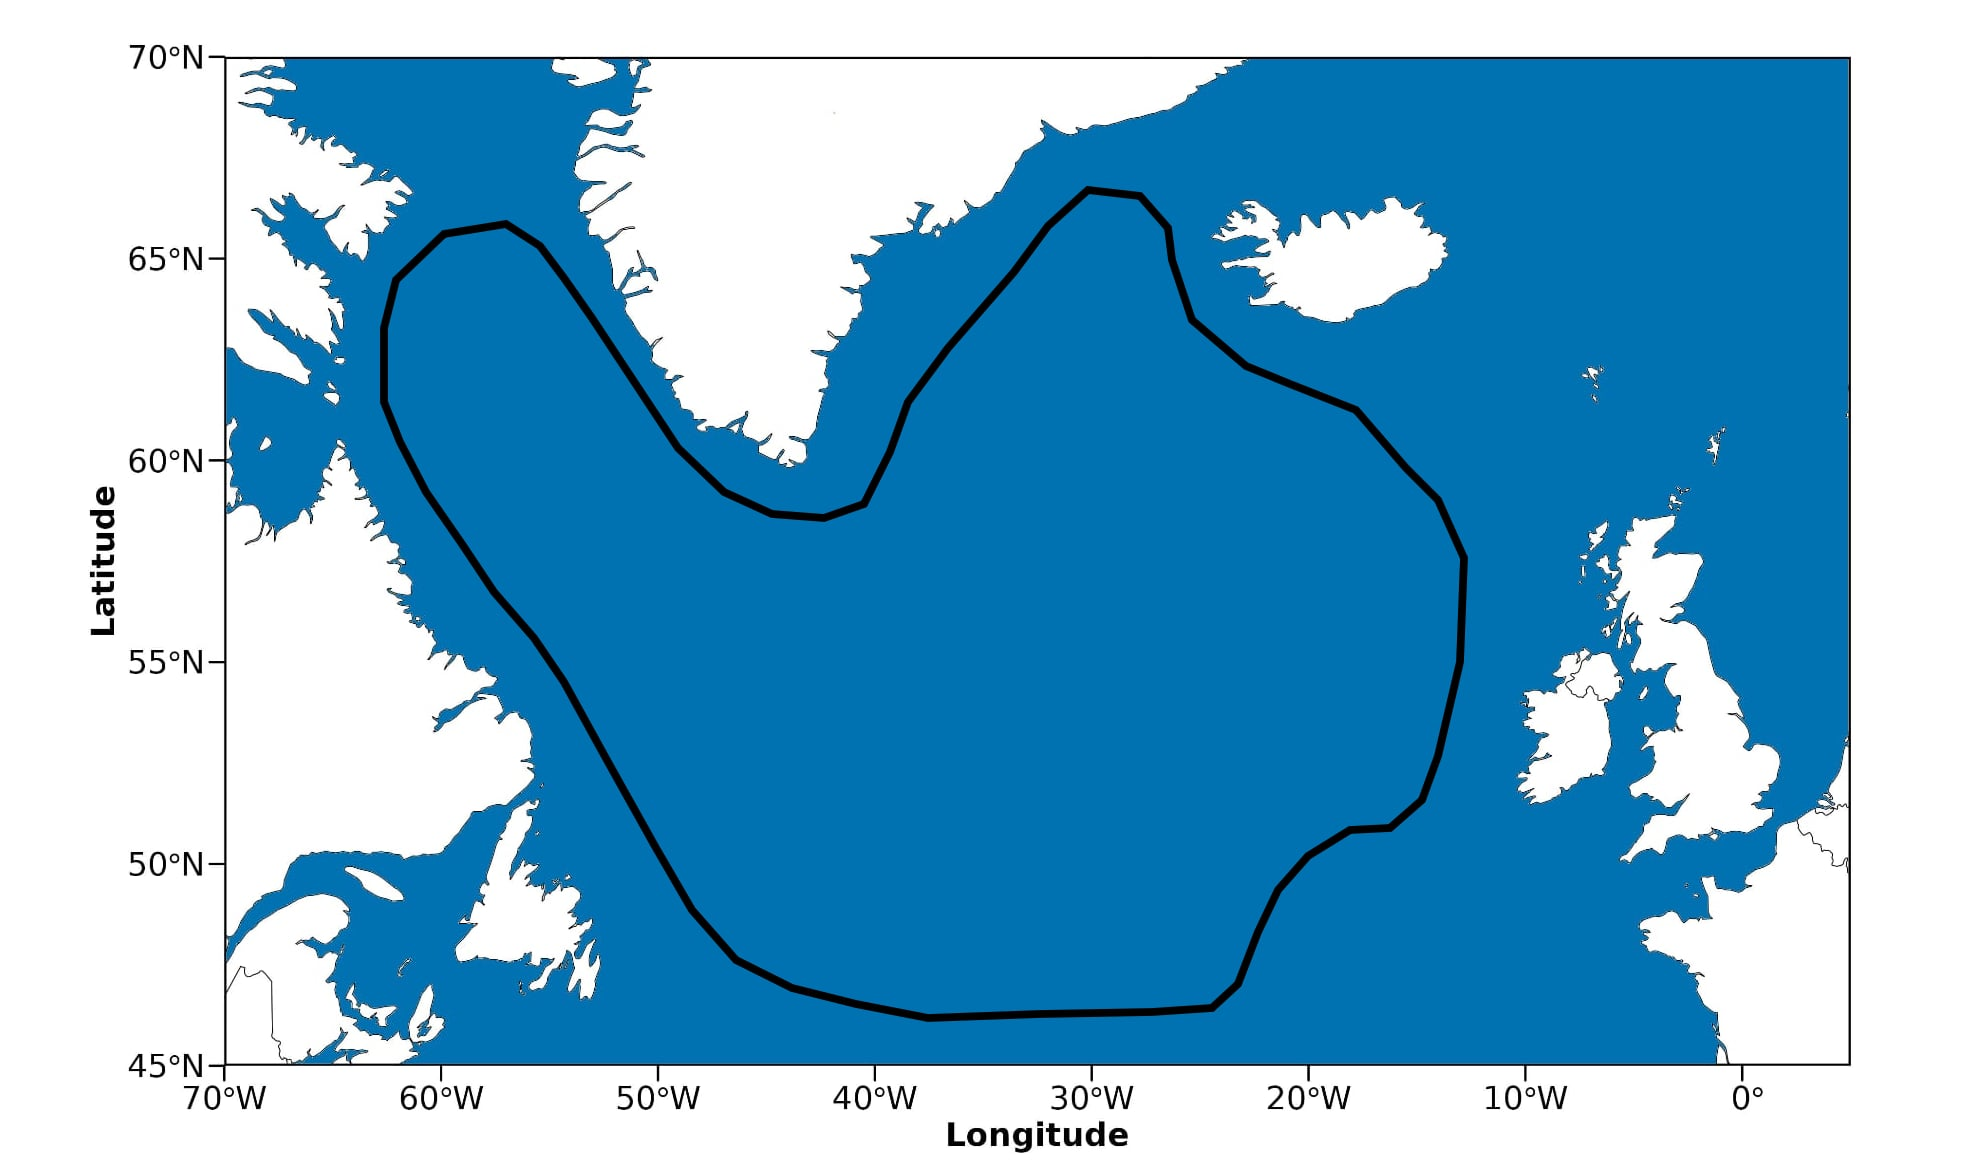
\includegraphics[scale = .175]{figures/NorthAtlanticOcean.jpeg}
    \end{center}
    \caption{The approximate location of the subpolar gyre in the North Atlantic Ocean}
    \label{figure:subpolarGyre}
\end{figure}\\
As the warm surface water moves north it loses heat due to the colder climate and because of mixing with other waters and evaporation, it becomes more saline. This increase in density causes the water to sink through convection, after which the water in the deep flows southward continuing the flow. 

Yet, in recent years there are indications of this process weakening. One driving factor is the increased melting of global ice sheets, particularly the Greenland ice cap, due to climate change. The influx of more freshwater in the area reduces the salinity of the water, which potentially hinders the sinking and thus disrupts the entire circulation. 

The strength of the AMOC has only been directly measured in the current millenium, which is not enough for our estimation methods to work. Instead, we consider time series of the mean sea surface temperature (SST) anomaly in the subpolar gyre (SG) in comparison to the global mean (GM) SST anomaly. These have been measured since $1870$ and the SG SST minus twice GM SST are largely agreed on proxy (or fingerprint) of the strength of the AMOC; in comparison to the rest of the world's oceans, there are in many places of the subpolar gyre an increasingly lower SST and this has been argued to be caused by the slowing down of the AMOC. Importantly note that the multiplication in the fingerprint is motivated by the amplification of global warming in the polar regions \cite[caption of Figure 1]{Ditlevsen2023}, which one would expect in this region.
\noindent We depict the time series of the mean SST temperature anomaly in the subpolar gyre as well as the global mean SST anomaly. At each time we also compute the AMOC fingerprint
\begin{figure}[h!]
    \begin{center}
    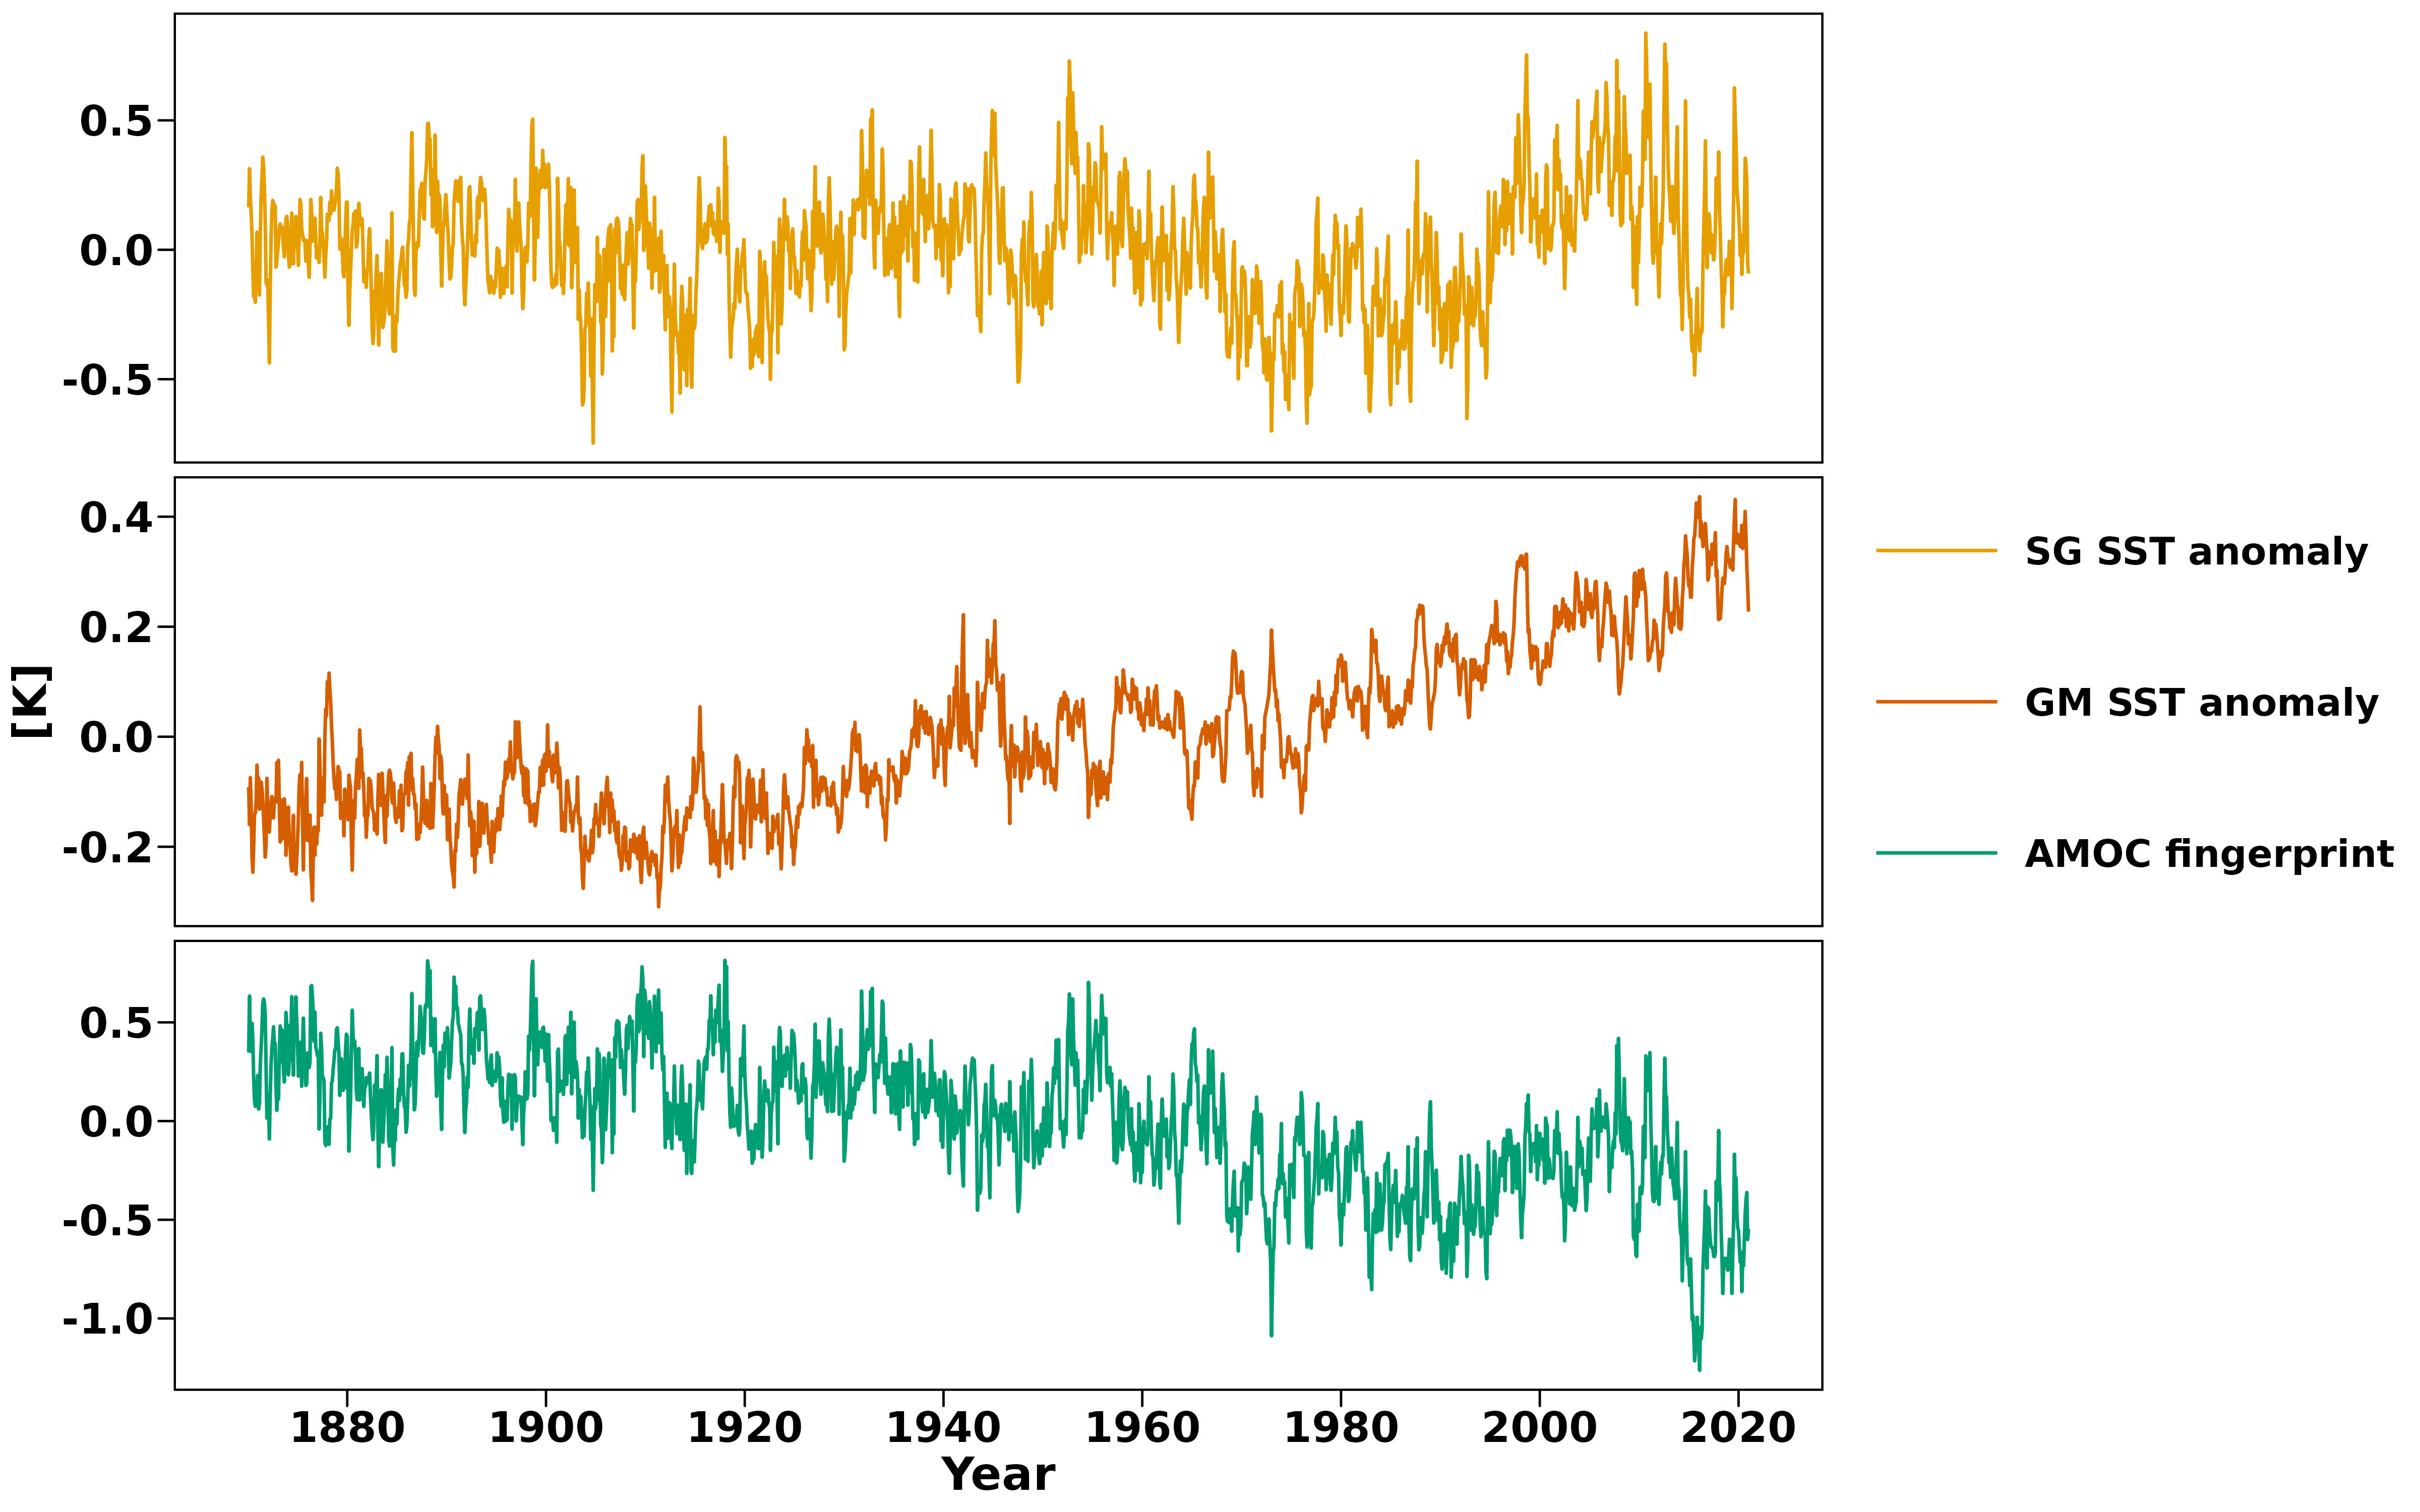
\includegraphics[scale = .06]{figures/AMOC_data_plot.jpeg}
    \caption{SST anomalies in the subpolar gyre and global mean as well as the AMOC fingerprint}
    \label{figure:AMOC_plot}
    \end{center}
\end{figure}\\
The fingerprint contains negative values, so without any transformations, we can only employ the additive- and $t$-diffusion-based models. The original work on these time series \cite{Ditlevsen2023} used a version of the additive model with penalization in the likelihood. Thus we try the $t$-diffusion-based model. Recall that the main qualitative difference between the models is that relative to the additive model the $t$-diffusion-based model has a stochastic term, which is always greater than or equal; other than that they are modelling the tipping in the same way. How the difference in diffusion term captures the AMOC-fingerprint remains to be seen though.
\subsubsection{Determining \texorpdfstring{$t_0$}{t0} and Estimating the AMOC Tipping Point}
We start by estimating parameters in the stationary- and dynamic parts of the process. Before we can do that we must figure out, which part of the time series we consider to be in the stationary- and dynamic part. Previous work found $t_0 = 1924$. This was done by a sweeping of the time of ramping, $t_0 \in [1910, 1950]$ used for a moment estimator of the tipping point; we do not consider this estimator in further detail, but instead propose an alternative method to arrive at the value of $t_0$ that does not depend on an extensive analysis of early warning signals. 

We sweep over the years $t_0 \in [1910, 1950]$ and split the data according to each $t_0$ and then estimate in the stationary - and dynamic parts. After this, we compare the normalized negative log-likelihoods of the different estimations with the number of observations in each part. We used the normalized objective because different $t_0$ results in different numbers of samples, causing us to favor models with more samples if we do not do this. Due to a lack of a better starting heuristic for the $t$-diffusion, we initialize the optimization of each of the stationary parts in the points corresponding to the approximate MLEs for the OU process \cite[equation (S4-S6)]{DitlevsenSupplementary}. While the initial values are meant for the OU process, the $t$-diffusion and it have the same one-step conditional mean and are qualitatively similar on the scale we are considering, so these initial values are at least somewhat justified.

In the different dynamic parts, we initialize the optimization in $A = 1$ and $\tau_c = 2021 - t_0$ for each of the $t_0$'s. The choice, $A = 1$ might seem a bit arbitrary, but with a lack of a better alternative it is made as it corresponds to a more parsimonious model. In addition, it is also the initial value of choice in the original application \cite{Ditlevsen2023}. Still, this heuristic only works because of the relatively small absolute values in the time series $\tau_c$ is chosen in the above way, because the values correspond to a lower bound for $\tau_c$. We have not observed tipping yet, thus $\tau_c$ is at least the difference between the largest year in the data: 2021 and the year when the initial ramping began. Sweeping over the years, we get a negative log-likelihood as a function of $t_0$ for the respective parts.
\begin{figure}[h!]
    \begin{center}
    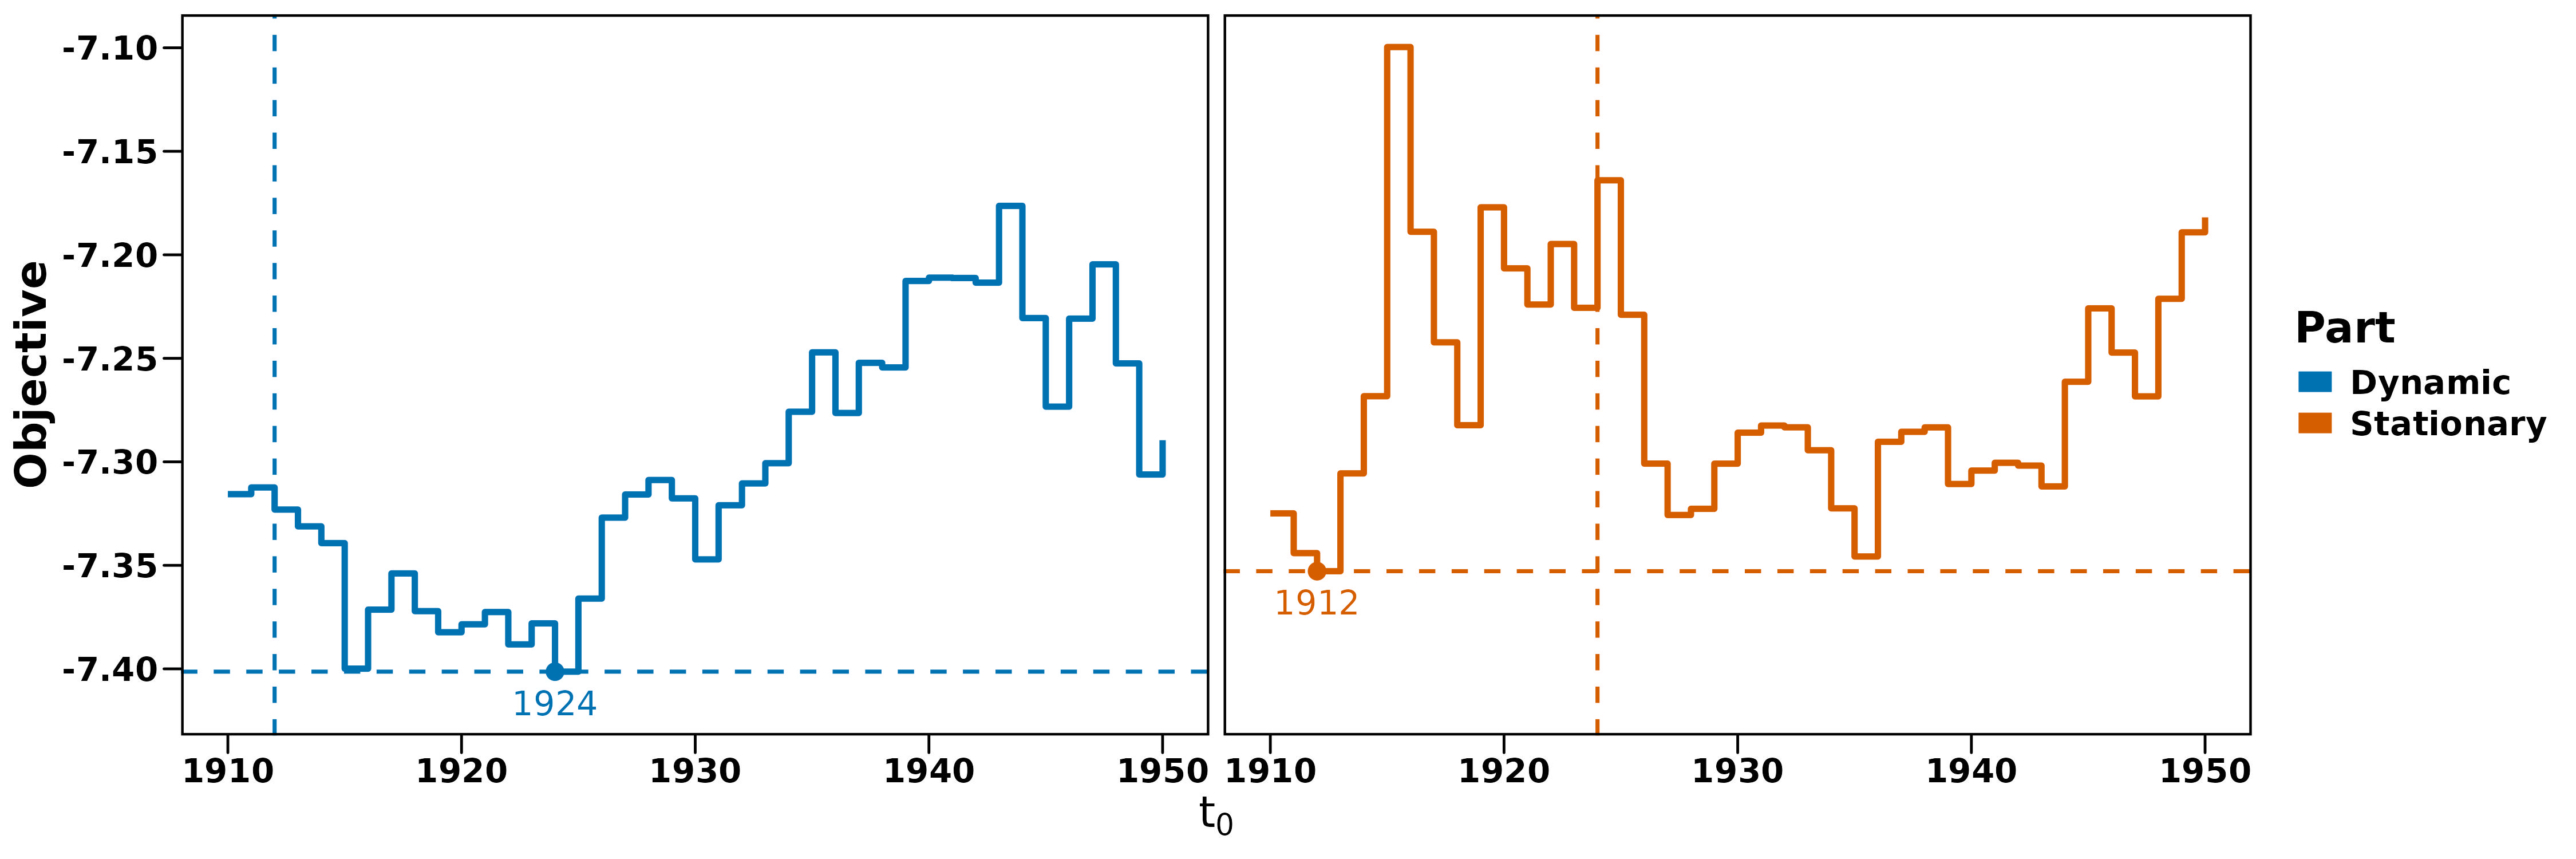
\includegraphics[scale = .095]{figures/ramping_year_likelihood_plot.jpeg}
    \caption{Negative log-likelihood for the stationary- and dynamic parts as a function of $t_0$.}
    \label{figure:negLoglikRamping}        
    \end{center}
\end{figure}\\
Where we have marked the minimal objective across all $t_0$ for both the stationary- and dynamic parts. Unfortunately, these are not the same value. To highlight this fact we have marked where the minimum is for one part onto the other by the vertical dotted lines. The horizontal lines are the values of the objective at the minimum $t_0$. Note that the $t_0$ that minimizes the objective for the dynamic part overall is the same as the one found in \cite{Ditlevsen2023}, i.e. $t_0 = 1924$. It is therefore tempting to pick this value, albeit we would like to be able to decide independently between the two. Another pitfall one could fall into is if one mistakenly assumes that there is any significance to the objective values being on similar scales numerically. They are, of course, different likelihoods and thus not comparable, meaning we cannot construct some sort of weighting between the two and select a middle-ground of sorts.
Considering this it seems that when the minima are this far away from each other, our method might seem to fall short. Before we go into details about how we might remedy this, let us quickly consider what impact the two different $t_0$'s have on the parameters. We take the estimated parameters from the sweep earlier and mark the two points in time where the stationary- and dynamic parts had their objectives minimized overall.
\begin{figure}[h!]
    \begin{center}
        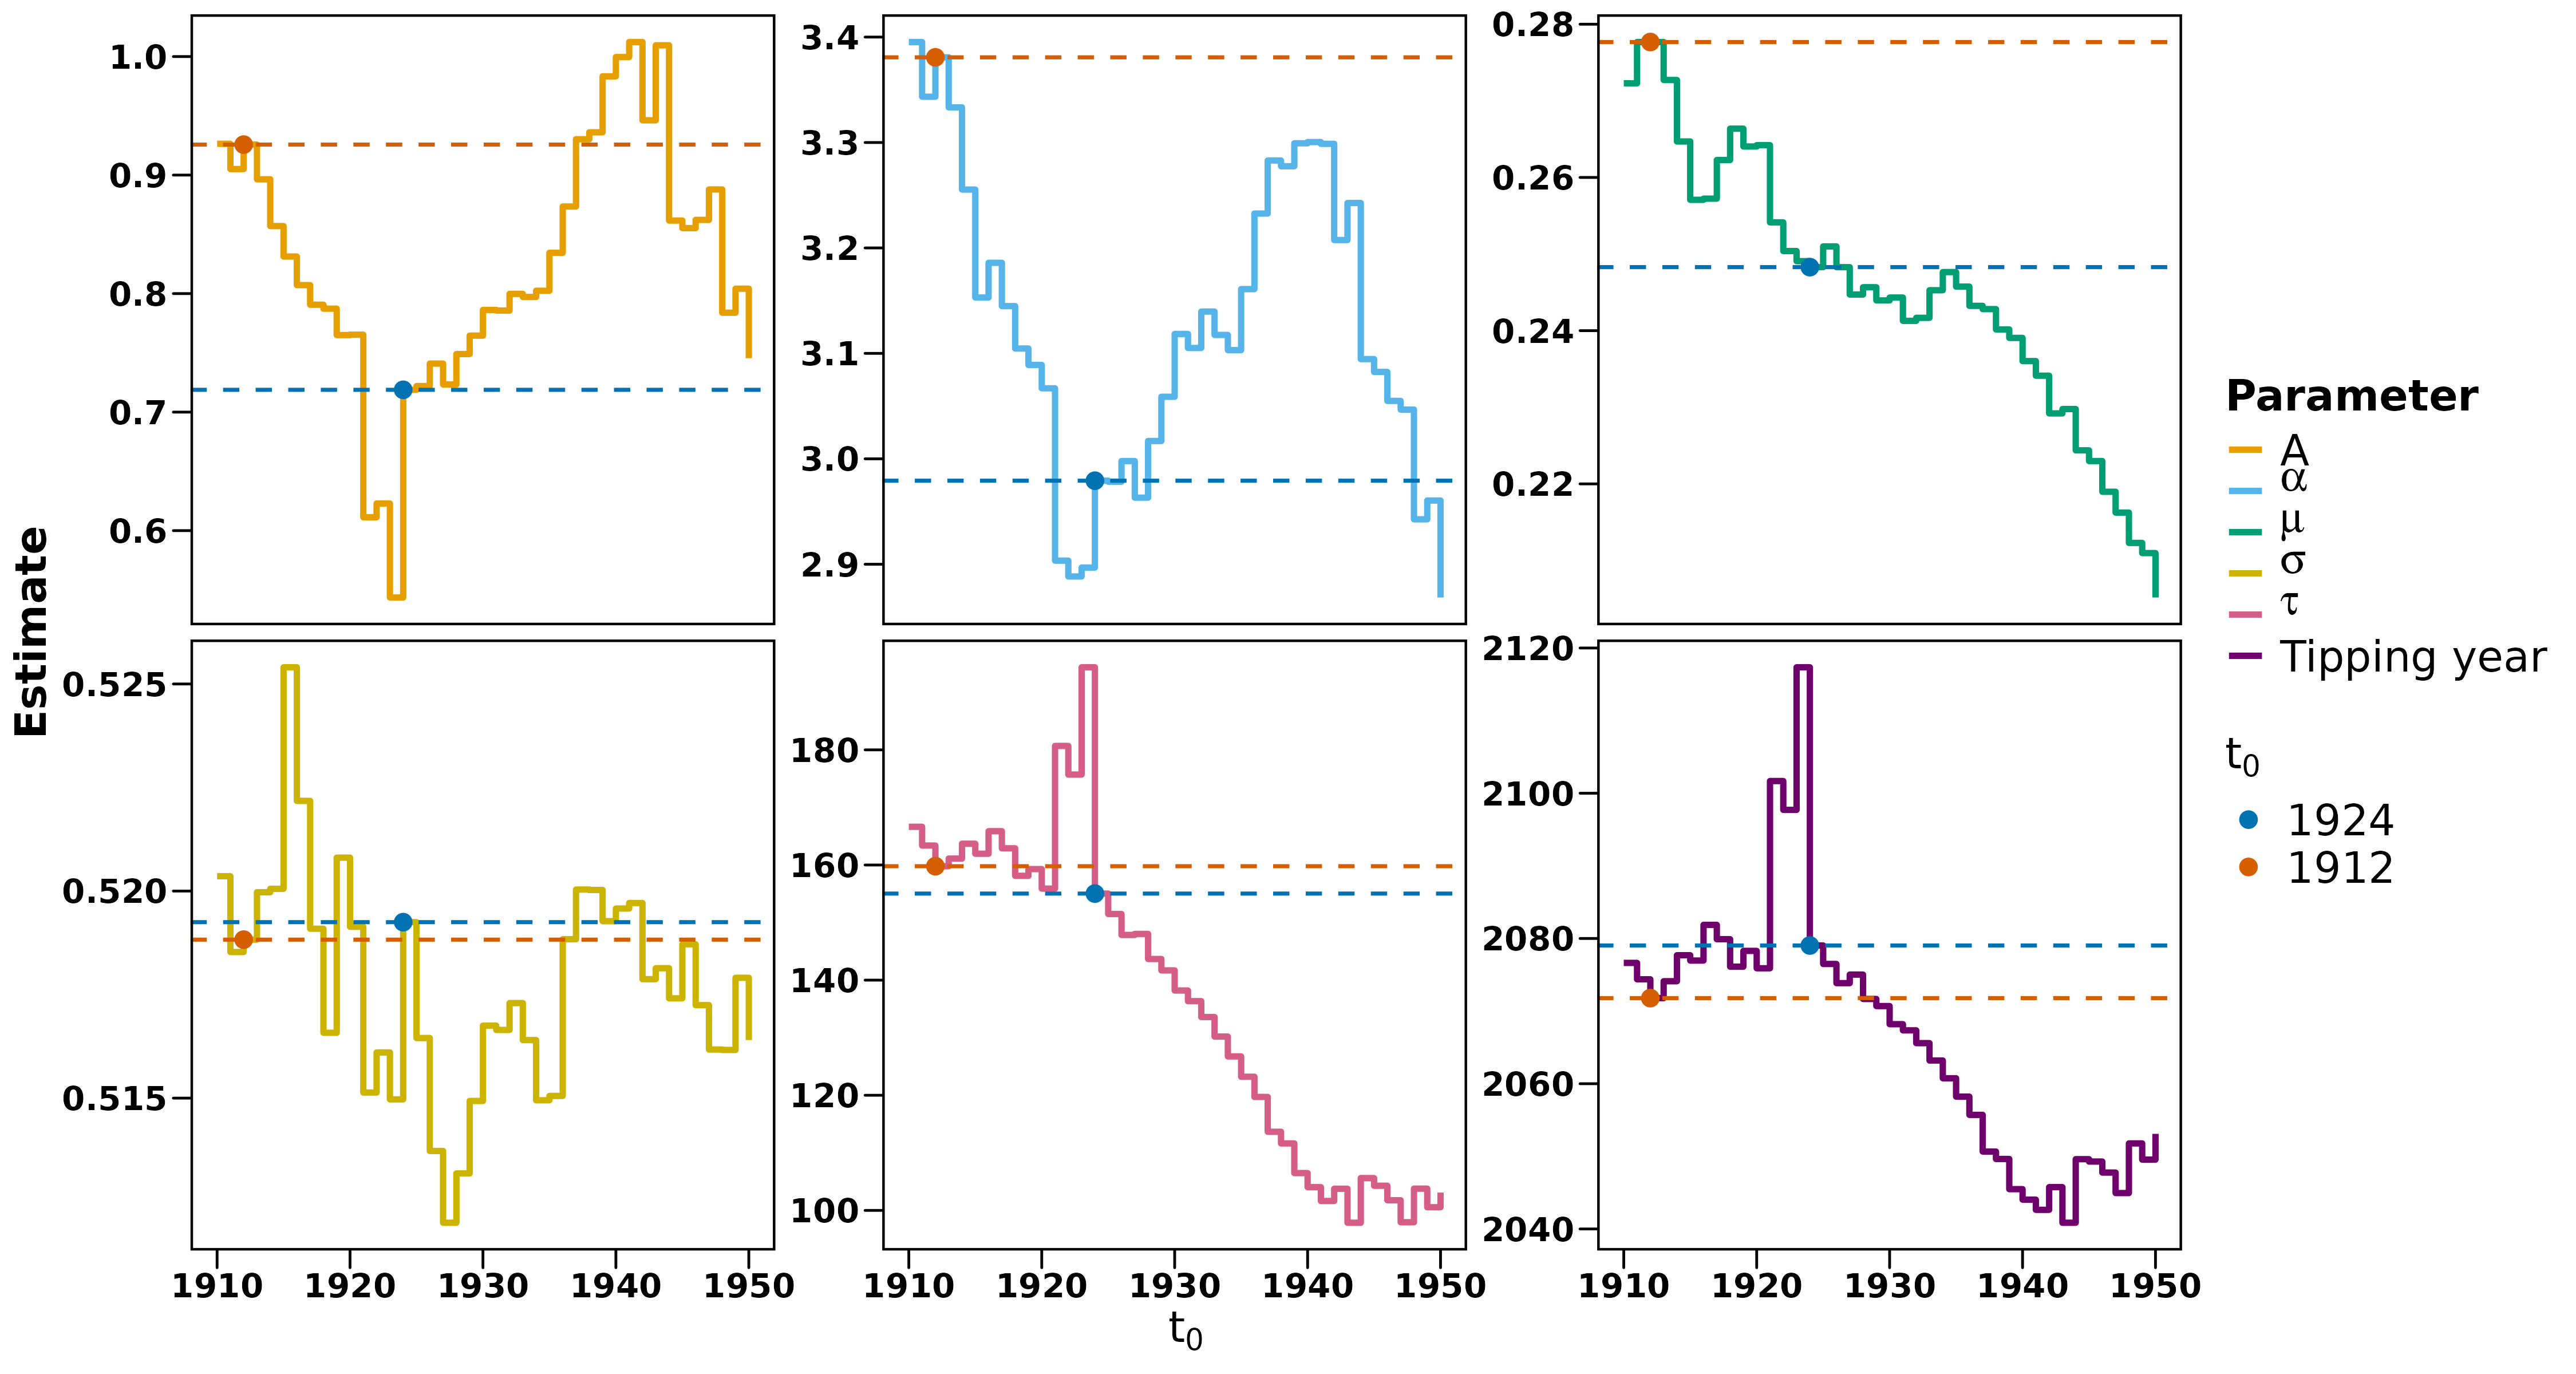
\includegraphics[scale = .09]{figures/estimators_full_plot.jpeg}
        \caption{Estimated values as a function of $t_0$ stratified after parameter — The values of $t_0$ that minimized the dynamic- and stationary objectives overall have been marked by points.}
    \end{center}
    \label{figure:AMOC_estimates_t_0}
\end{figure}\\
Generally, the estimates from the two models seem to mostly agree. Of course, we have to consider the scale of the individual estimates to say this for sure. To compare we tabularize the respective estimates at the two points and their relative differences
\begin{table}[h!]
    \centering
    \begin{tabular}{lllr}
     Parameter & Estimates 1924 & Estimate 1912 & Relative difference \\ \hline
    $\alpha_0$ & $2.98$ & 3$.38$ & $-11.88\%$ \\ 
      $\mu_0$ & $0.25$ & $0.28$ & $-10.58\%$ \\ 
      $\sigma$ & $0.52$ & $0.52$ & 0$.08\%$ \\ 
      $\tau_c$ & $155.03$ & $159.79$ & $-2.98\%$ \\ 
      Tipping year & $2079.03$ & $2071.79$ & $0.35\%$\\ 
      $A$ & $0.72$ & $0.93$ & $-22.35\%$ \\ 
       \hline
    \end{tabular}
    \caption{Parameter estimates from the stationary- and dynamic parts for the $t$-diffusion-based model of the normal saddle-node form stratified after whether ramping time to minimize the stationary- or dynamic negative log-likelihood is used.}
    \label{table:Estimates_t0_AMOC}
\end{table}\\
Though it might already have been clear from Figure \ref{figure:AMOC_estimates_t_0}, Table \ref{table:Estimates_t0_AMOC} clearly indicates that the parameters $A, \alpha_0, \mu_0$ deviate more from one another between the two $t_0$'s than the remaining parameters. To this end, it is positive that the $\tau_c$-parameters, and additionally the tipping years have a very small relative difference. Interestingly, due to the different values of $t_0$ the tipping years are almost equal in spite of the $\tau_c$-parameters being more different, relatively speaking. This is naturally good news as it seems that the two models are almost in perfect agreement on the most important aspect of our modelling. Still, we seek to find \textit{the} ramping time and to do so we diagnose the two models with uniform residuals for both the stationary- and dynamic part of the process for both $t_0$ and plot the Q-Q plots for each part stratified after which $t_0$ was used.
\begin{figure}[h!]
    \begin{center}
        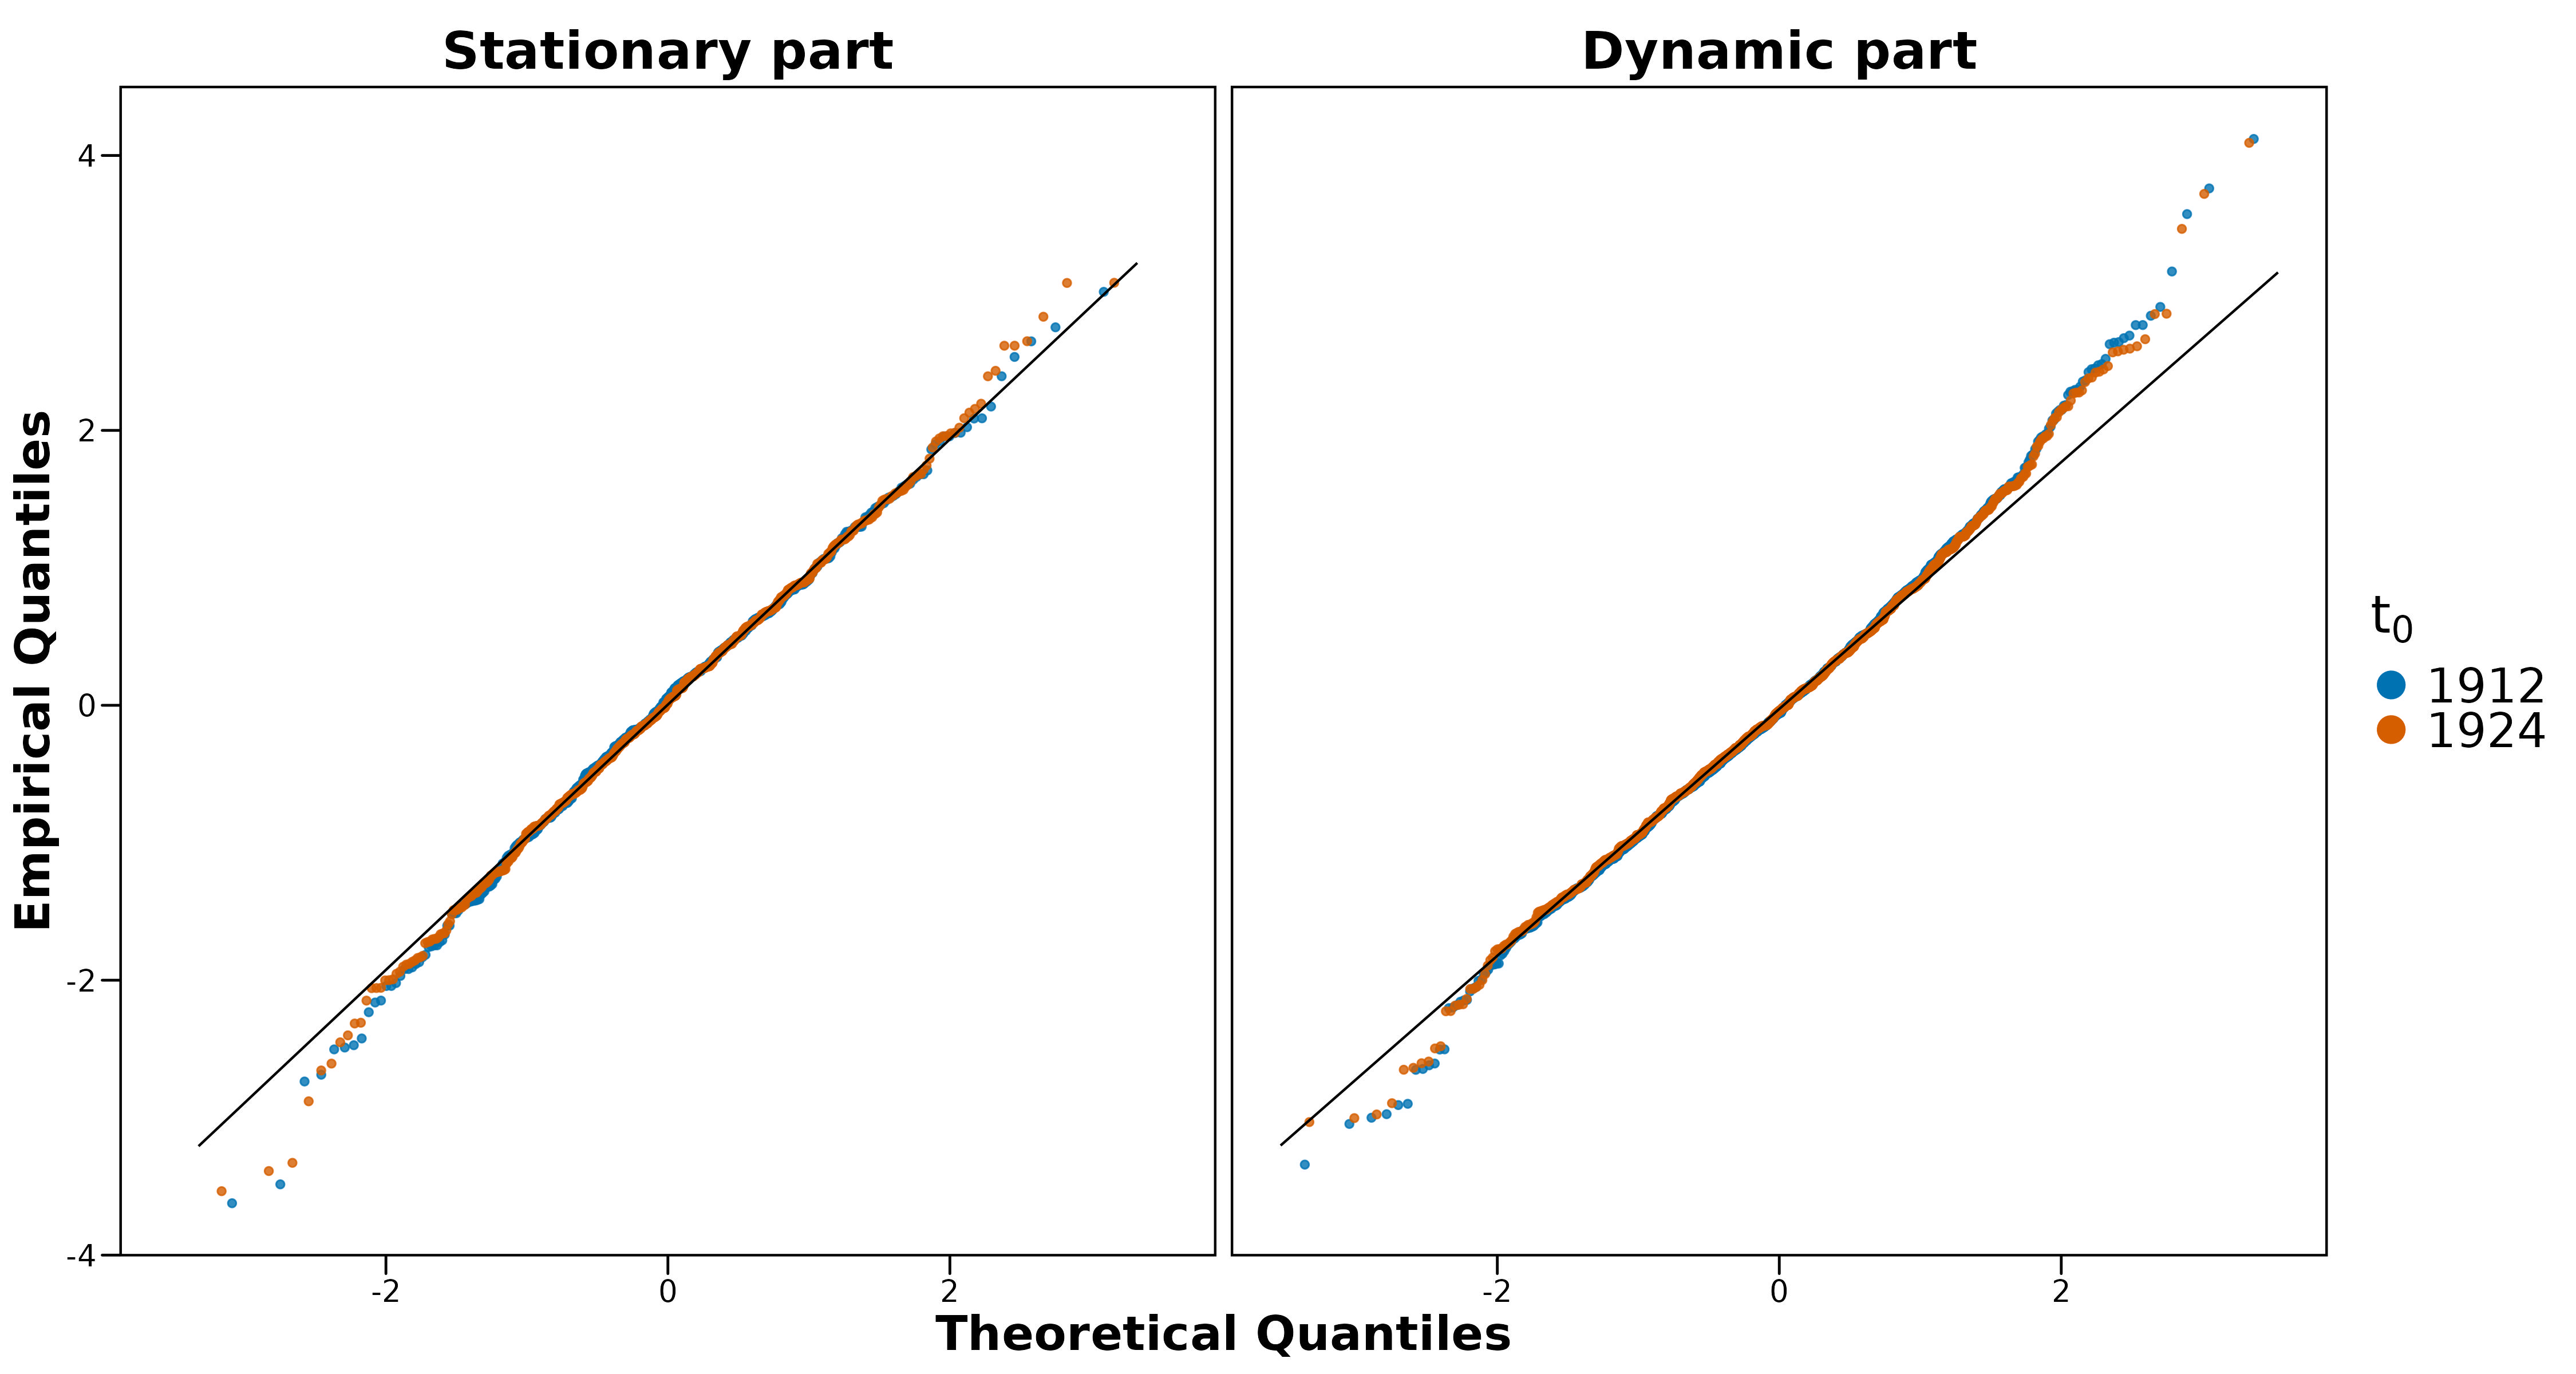
\includegraphics[scale = .09]{figures/QQ_plot_parts.jpeg}
        \caption{Q-Q plots for the stationary- and dynamic parts grouped by the $t_0$ used.}
        \label{figure:AMOC_QQ_t_0}
    \end{center}
\end{figure}\\
Looking at the Q-Q plot for the stationary part, we unsurprisingly see that the fit corresponding to $t_0 = 1912$ appears a bit better, albeit the two are hard to distinguish. Generally though, the empirical quantiles seem a bit heavy-tailed suggesting a slight lack of fit. Conversely, the fit in the dynamic part appears to be better when using $t_0 = 1924$. The difference between the two ramping values seems to be more pronounced here. Sometimes it can be a bit difficult to diagnose these fits due to a couple of extreme outliers. To illustrate this we tabularize the empirical quantiles and add the theoretical quantiles from the standard normal distribution. In the core of the distributions, there is not too big of a difference between the two $t_0$; though the overall impression is the same, so we move on with $t_0 = 1924$ and refer to Table \ref{table:QQ_table_parts} in Appendix \ref{section:benchmark} for the exact quantiles.\newpage 
\subsubsection{Model evaluation and Confidence intervals for the Estimates}
Although we already have presented our diagnostics of choice for the model in advance qua the uniform residuals in Figure \ref{figure:AMOC_QQ_t_0}, we have yet to assess the uncertainty of the parameters. Recall that our estimates correspond to the values in the \textit{"Estimates 1924"}-column in Table \ref{table:Estimates_t0_AMOC}. We simulate using the $t$-diffusion-based scheme in (\ref{eq:skew_t_sim}) with these parameters. Then we fit the model to the simulated data with the estimated parameters from the original data set as the starting values. Simulating $M = 2000$ realizations from the model and estimating in the respective parts, we get the following distribution of the estimates
\begin{figure}[h!]
    \begin{center}
    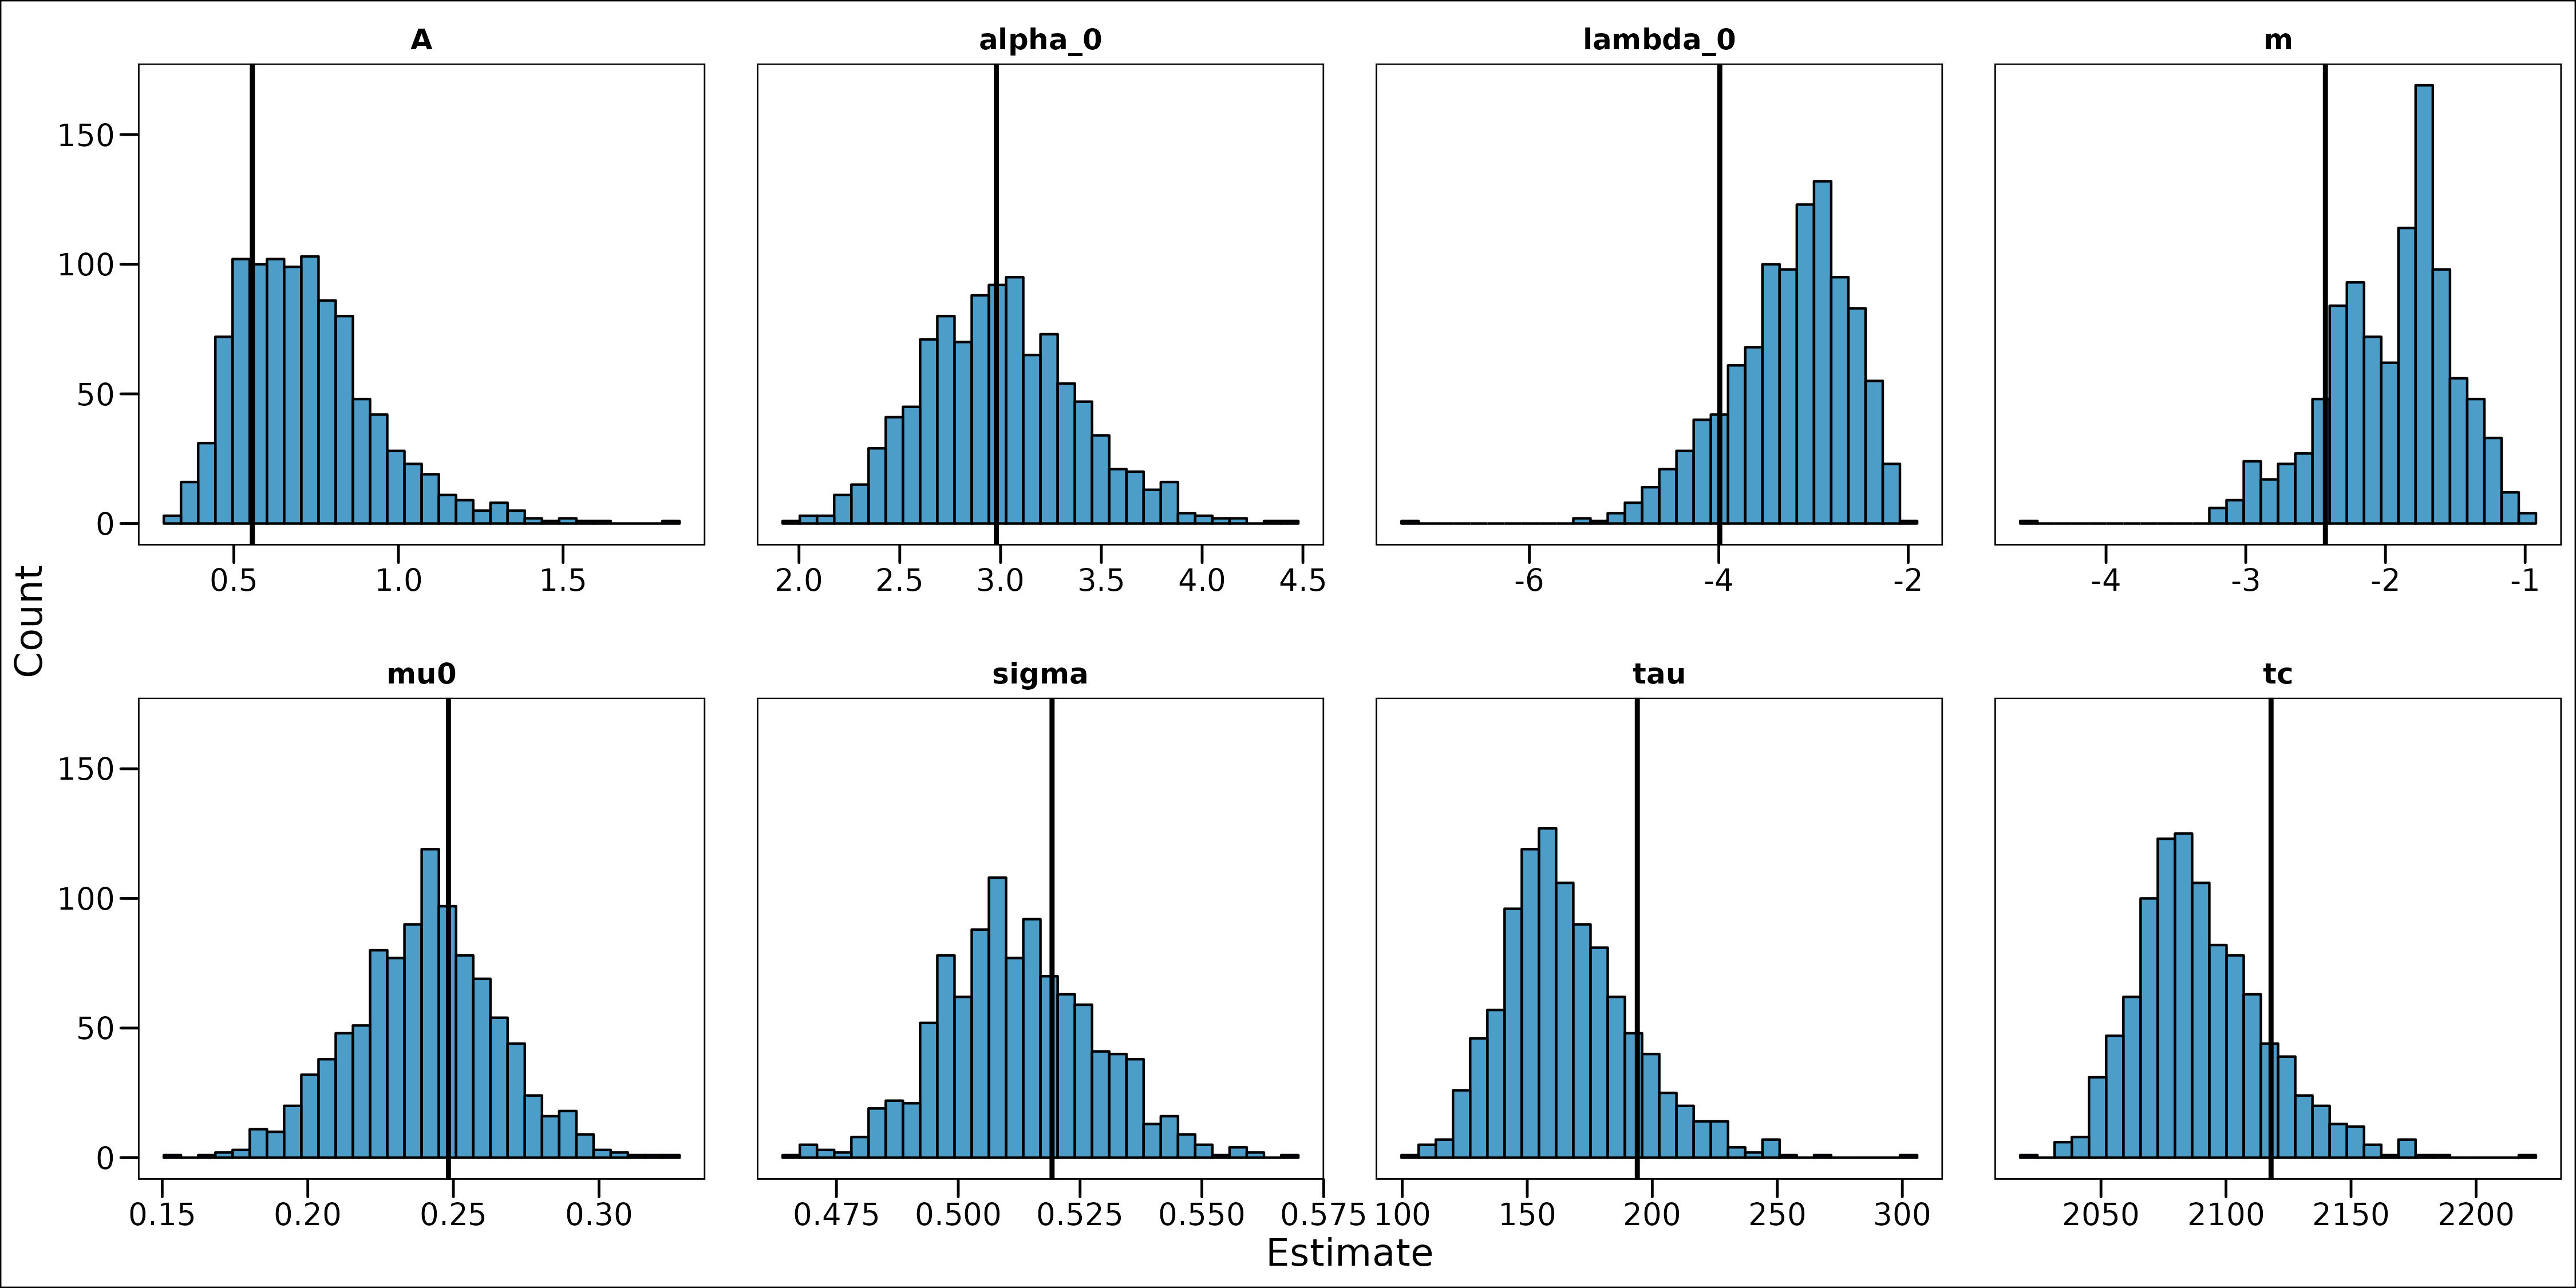
\includegraphics[scale = .095]{figures/estim_tibble_plot.jpeg}
    \caption{Normalized histograms of the estimates from the $t$-diffusion-based bifurcation tipping model made with parametric bootstrap.}
    \label{figure:AMOC_parametric_bootstrap}
    \end{center}
\end{figure}\\
In the histograms, the estimates from the original fit to the AMOC data have been overlayed with a dashed line for the respective parameters. Note that for a clearer impression of the distribution, we have removed $7$ extreme estimates of the total $2000$. These estimates have been tabularized and can be seen in Appendix \ref{section:benchmark} in Table \ref{table:extreme_amoc_estimates}. All the empirical distributions of the estimates cover the values that we estimated from the original data well cementing what we have already seen qua the uniform residuals — that there is an overall good fit to the data.
\subsection{Robustness Analysis and The Additive noise model}
In this section we repeat the analysis from before but here we look into other choices of fingerprint for the AMOC. We follow the idea presented in \cite{Ditlevsen2023}. The two alternative fingerprints are the SST temperature anomaly in the subpolar gyre minus respectively one or three times the global mean SST anomaly.

Recall the original AMOC fingerprint was defined as the SST temperature anomaly in the subpolar gyre minus \textit{two} times the global mean SST anomaly. The original work on the subject coined the terms \textit{AMOC1}, \textit{AMOC2} and \textit{AMOC3} for the respective fingerprints referencing the factor in front of the global mean SST anomaly. For a visual representation of the difference between the fingerprints refer to Figure \ref{figure:allAMOCFingerprints}.\\\\
We repeat the estimation and parametric bootstrap from the previous section on each of the alternative fingerprints. For each fingerprint, we find the corresponding $t_0$ using the same methods as above. The parametric bootstraps were again done by sampling $M = 2000$ times from the respective models and estimating in the simulated time series. Here we only present the distribution of the tipping year as this is our parameter of interest, but the remaining results can be found in Appendix \ref{subsubsec:RobustnessAnalysisAppendix} too. In addition to the fit of the AMOC1 and AMOC3, we also try using the model with additive noise. Recall that unlike \cite{Ditlevsen2023} our estimation does not use penalization on $A$ in the estimation of the dynamic part of the process, so the models are not completely the same. We summarize our findings in the following table and graph
\begin{table}[ht]
    \centering
    \begin{tabular}{rrrrrrrr}
    Model & Fingerprint & Estimate    & 0.025  & 0.165  & 0.5    & 0.835  & 0.975 \\ 
      \hline
    Additive & AMOC1 & 2120.9         & 2076.9 & 2106.5 & 2138.8 & 2169.8 & 2236.4 \\
    Additive & AMOC2 & 2077.9         & 2039.7 & 2053.5 & 2080.5 & 2113.2 & 2150.8 \\ 
    Additive & AMOC3 & 2088.3         & 2036.2 & 2056.1 & 2090.6 & 2121.7 & 2146.8 \\ \hline 
    t-diffusion & AMOC1 & 2093.1      & 2054.3 & 2075.2 & 2103.2 & 2135.2 & 2190.4 \\ 
    t-diffusion & AMOC2 & 2079.0      & 2039.7 & 2054.6 & 2083.7 & 2117.1 & 2157.1 \\ 
    t-diffusion & AMOC3 & 2101.0      & 2037.5 & 2070.9 & 2102.5 & 2131.9 & 2152.9 \\ 
    \hline 
    Pen. additive& AMOC1 & 2083       & 2024 & 2062 & - & 2128 & 2180 \\
    Pen. additive& AMOC2 & 2057       & 2025.3 & 2039.0 & 2052.6 & 2069.9 & 2095.1 \\ 
    Pen. additive& AMOC3 & 2067       & 2034 & 2048 & - & 2083 & 2102 \\
       \hline
    \end{tabular}
    \caption{Selected quantiles for the tipping year stratified after which model and type of fingerprint we used. In addition, the parametric bootstrap from the original analysis \cite{Ditlevsen2023} is included.}
    \label{table:tipping_quantiles}
\end{table}\\
The table shows the same quantiles of the tipping year as \cite{DitlevsenSupplementary}; the \textit{Pen. additive} Model corresponds to the model from \cite{Ditlevsen2023}. Note that in this study bootstrapping was done with $M = 1000$. Additionally note that \cite[Table 1]{Ditlevsen2023} gives $66$- and $95\%$ confidence intervals for the tipping year for the penalized additive model using the AMOC1 and AMOC3 fingerprint, whereas the complete distribution was found for the AMOC2 fingerprint in \cite{DitlevsenSupplementary}.\newpage 
\noindent To present the same information in perhaps a more illustrative way we plot the survival curves of the tipping year estimates stratified after model and fingerprint
\begin{figure}[h!]
    \begin{center}
        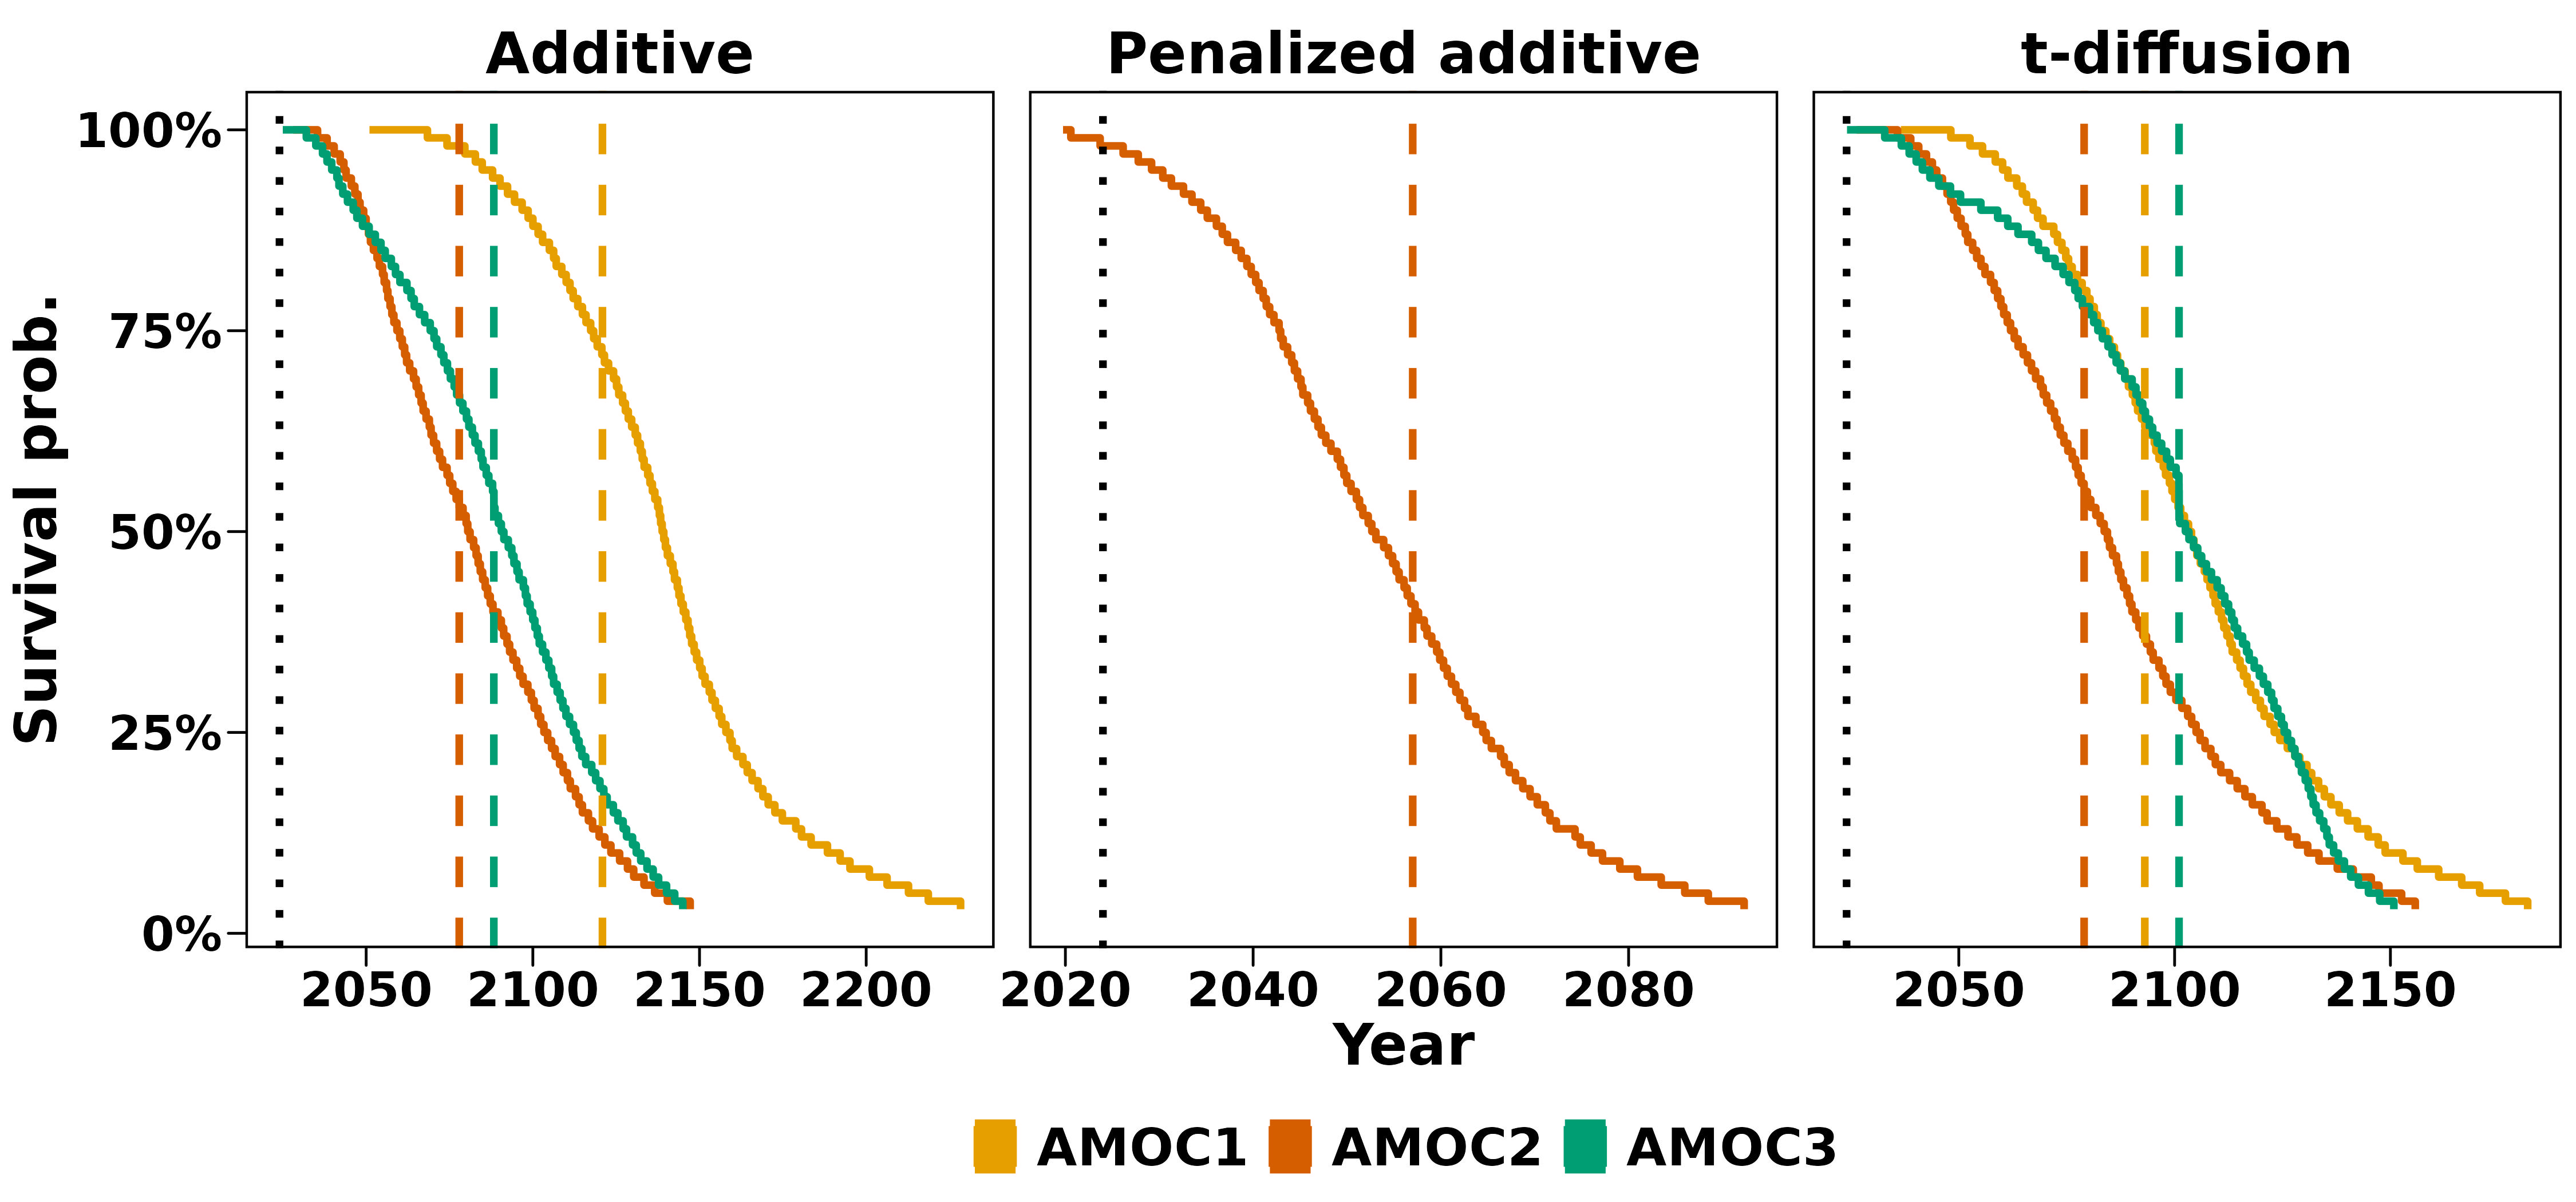
\includegraphics[scale = .096]{figures/surival_curve_first97.5.jpeg}
        \caption{The distribution of the tipping year stratified after model and type of fingerprint used — illustrated as the survival curve of the tipping year.}
        \label{figure:surival_curve_taus}
    \end{center}
\end{figure}\\
The black dotted line marks the current year, $2024$ and the colored dashed line is the estimated tipping year from the AMOC data. To be completely clear, Figure \ref{figure:surival_curve_taus} gives, according to the models, the probability that tipping has not occurred in a given year. And for the sake of readibility, we have removed the $2.5\%$ most extreme observations at the higher end of the years.\\\\
Unfortunately, we could not find the distributions for AMOC1 and AMOC3 in the penalized additive model, so we cannot construct the curves for these fingerprints. However, Table \ref{table:tipping_quantiles} clearly shows the robustness of the methods employed in \cite{Ditlevsen2023}. With regards to our own methods, the tipping years seem quite robust both against choice of model i.e. choice of stochastic term and choice of fingerprint. In the inter-model comparison, the difference between the quantiles in the two models for a specific type of fingerprint is miniscule. On the intra-model side of things, the estimates do not deviate too much from one another either. Yet, our models give estimates that are quite heavy-tailed in comparison with the penalized additive model.
\newpage
\noindent Finally, we show a direct comparison between the uniform residuals of the two models
\begin{figure}[h!]
\begin{center}
    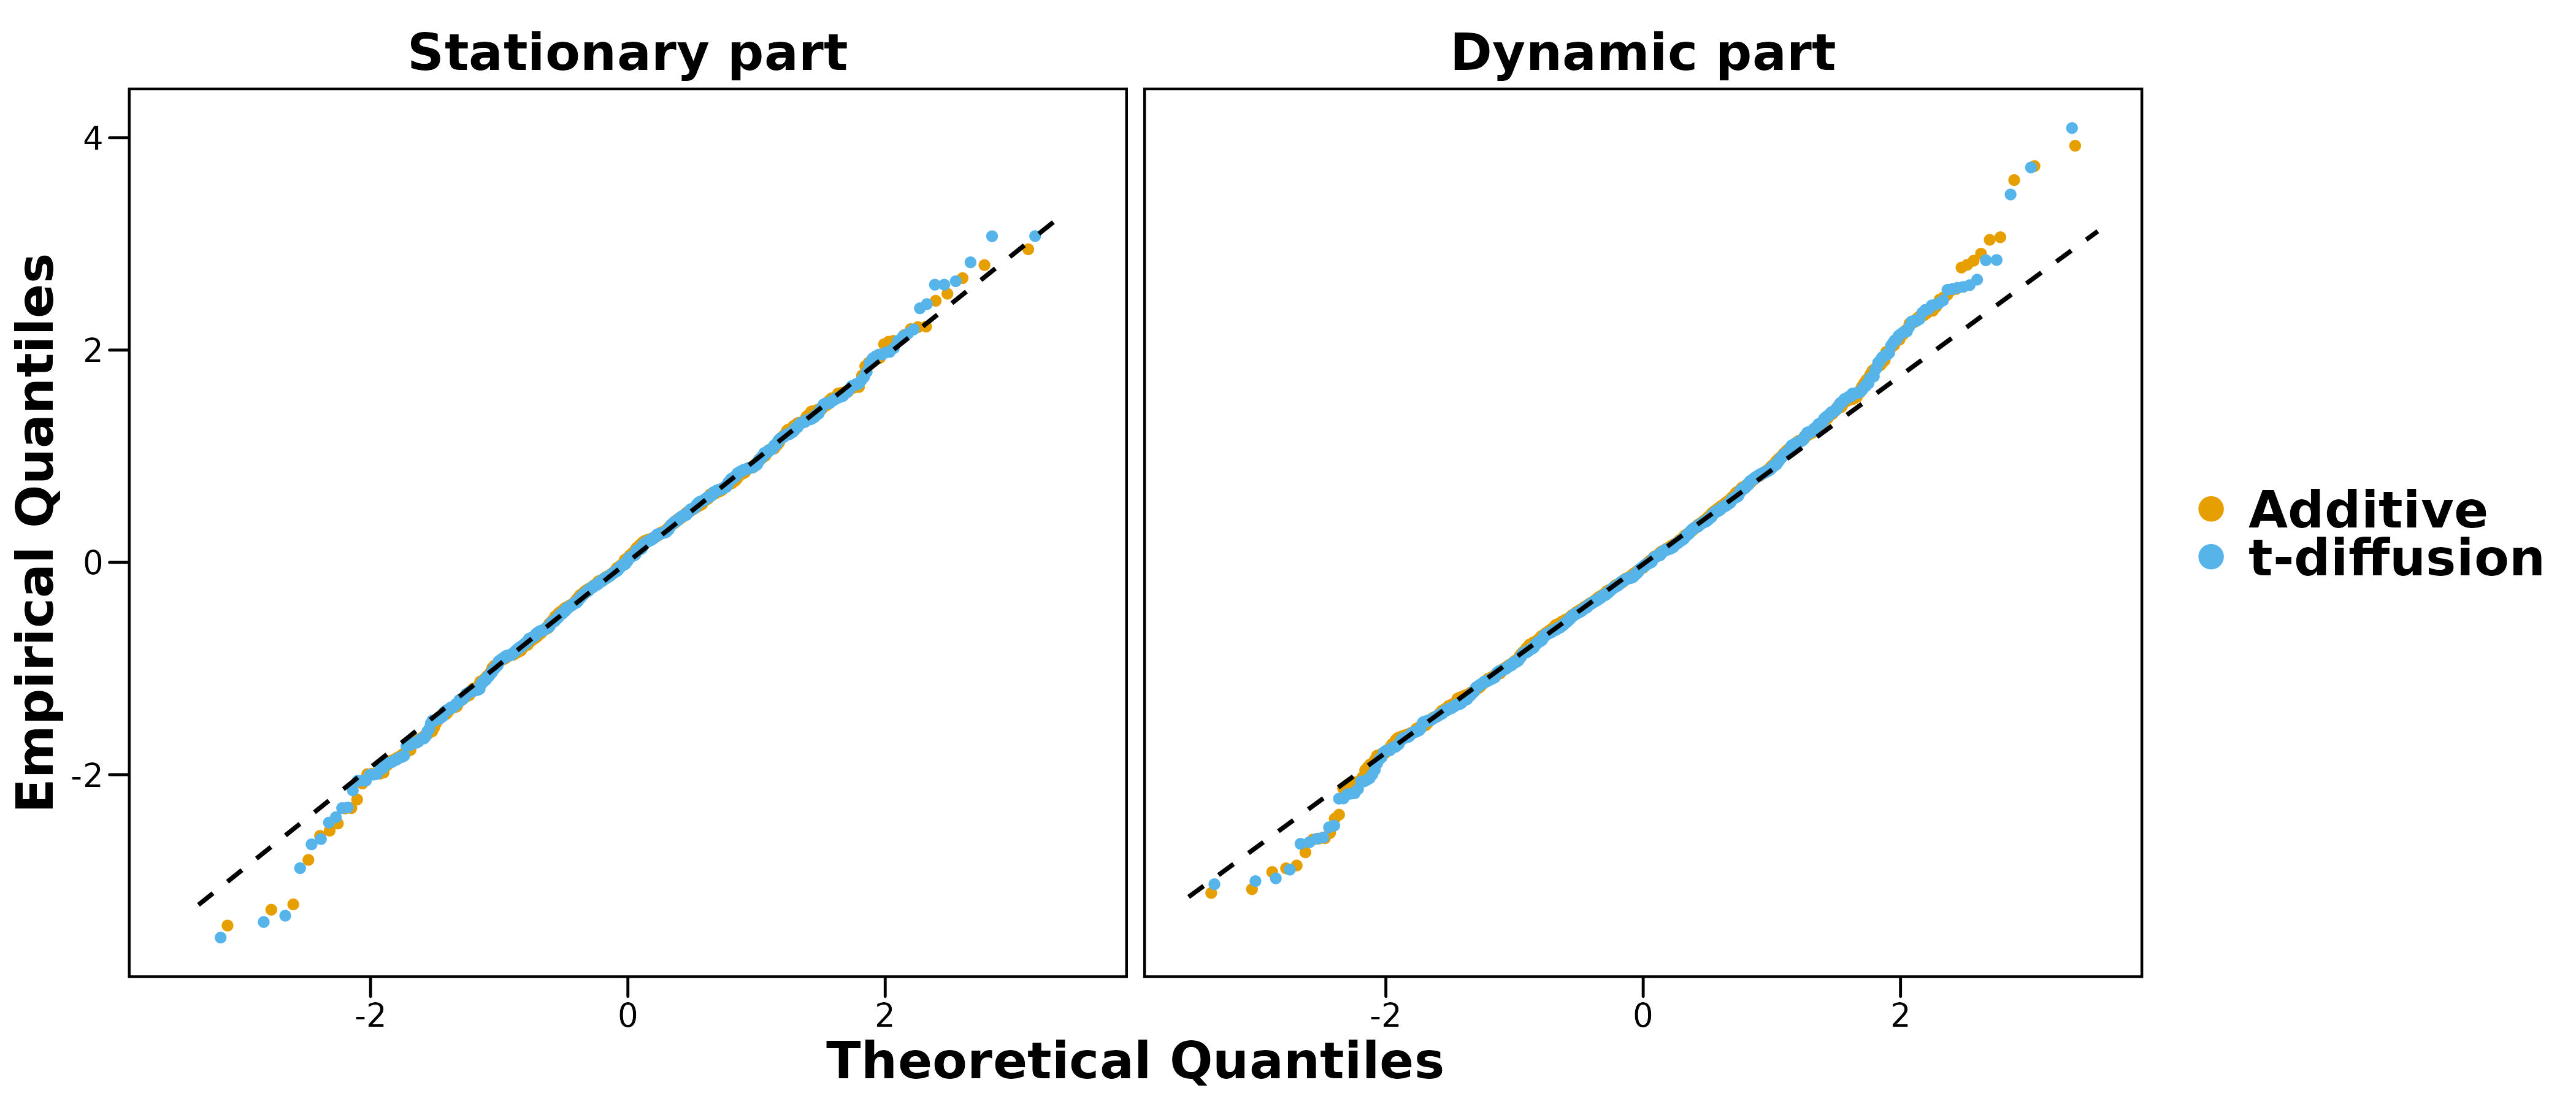
\includegraphics[scale = .1]{figures/OU_vs_t_diffusion_QQ_plot.jpeg}
    \caption{Empirical quantiles of the uniform residuals stratified after part of the process and which model was fitted.}
    \label{figure:OU_t_diffusion_QQ_plot}
\end{center}
\end{figure}\\
The overall impression of Figure \ref{figure:OU_t_diffusion_QQ_plot} is that the models are indistinguishable in the stationary part, whereas the $t$-diffusion-based model has a slight edge in the tails in the dynamic part. Though they are both a bit heavy-tailed in comparison with the standard normal quantiles. However, this happens mostly in the far end of the tails. 

As said earlier, it can sometimes be a bit difficult to differentiate models on these graphs. In Table \ref{table:QQ_OU_vs_t_diffusion} in Appendix \ref{subsubsec:RobustnessAnalysisAppendix} we illustrate select quantile values of the uniform residuals in Figure \ref{figure:OU_t_diffusion_QQ_plot} to support the claims made here. Looking at the Table, the stationary part of the process is captured a bit better by the additive model, while the opposite is true for the dynamic part. According to the Table, all quantiles of the uniform residuals from the $t$-diffusion-based model but the $0.975$-quantile are closest to the corresponding quantile in the standard Gaussian distribution.
% \subsection{Tipping in global climate variations}
% Climate physicists have extensively studied ice core data from Greenland as the Greenland ice sheet acts as a sediment for the atmosphere. It is widely accepted that the ratio between the isotopes $^{18}\mathrm{O}$ and $^{16}\mathrm{O}$ is an indicator of the temperature at the time of accumulation. Additionally, $\mathrm{Ca}^{2+}$-ions from dust settle in the ice layer by layer. Unlike the ratio they do not diffuse as much; this allows us to have a finer temporal resolution. We can use calcium-ions instead of the ratio, because there is a negative correlation betwen the logarithm of the log-concetration of the $\mathrm{Ca}^{2+}$-ions and the isotope-ratio. This means that higher calcium-ion concentrations indicate colder global conditions. The ice-core data consists of observations of the oxygen isotope ratio and $\mathrm{Ca}^{2+}$-ion concentrations from $107620$ years before present to $10260$ years before present with a constant temporal resolution of $20$ years. We rescale to kilo years and focus on the observation of the calcium-ion between $86$ kilo years before present (kyrs bp) and $55$ kyrs bp; of course still with $\Delta t = 0.02$. Now, transforming ion-concentrations by $-\log (x)$ is a common practice in chemistry, whence we also consider $-\log([\mathrm{Ca}^{2+}]) - C$, where $C$ is a constant that makes the process have mean zero. We depict the ion-concetration over time. 
% \begin{figure}[h!]
%     \begin{center}
%     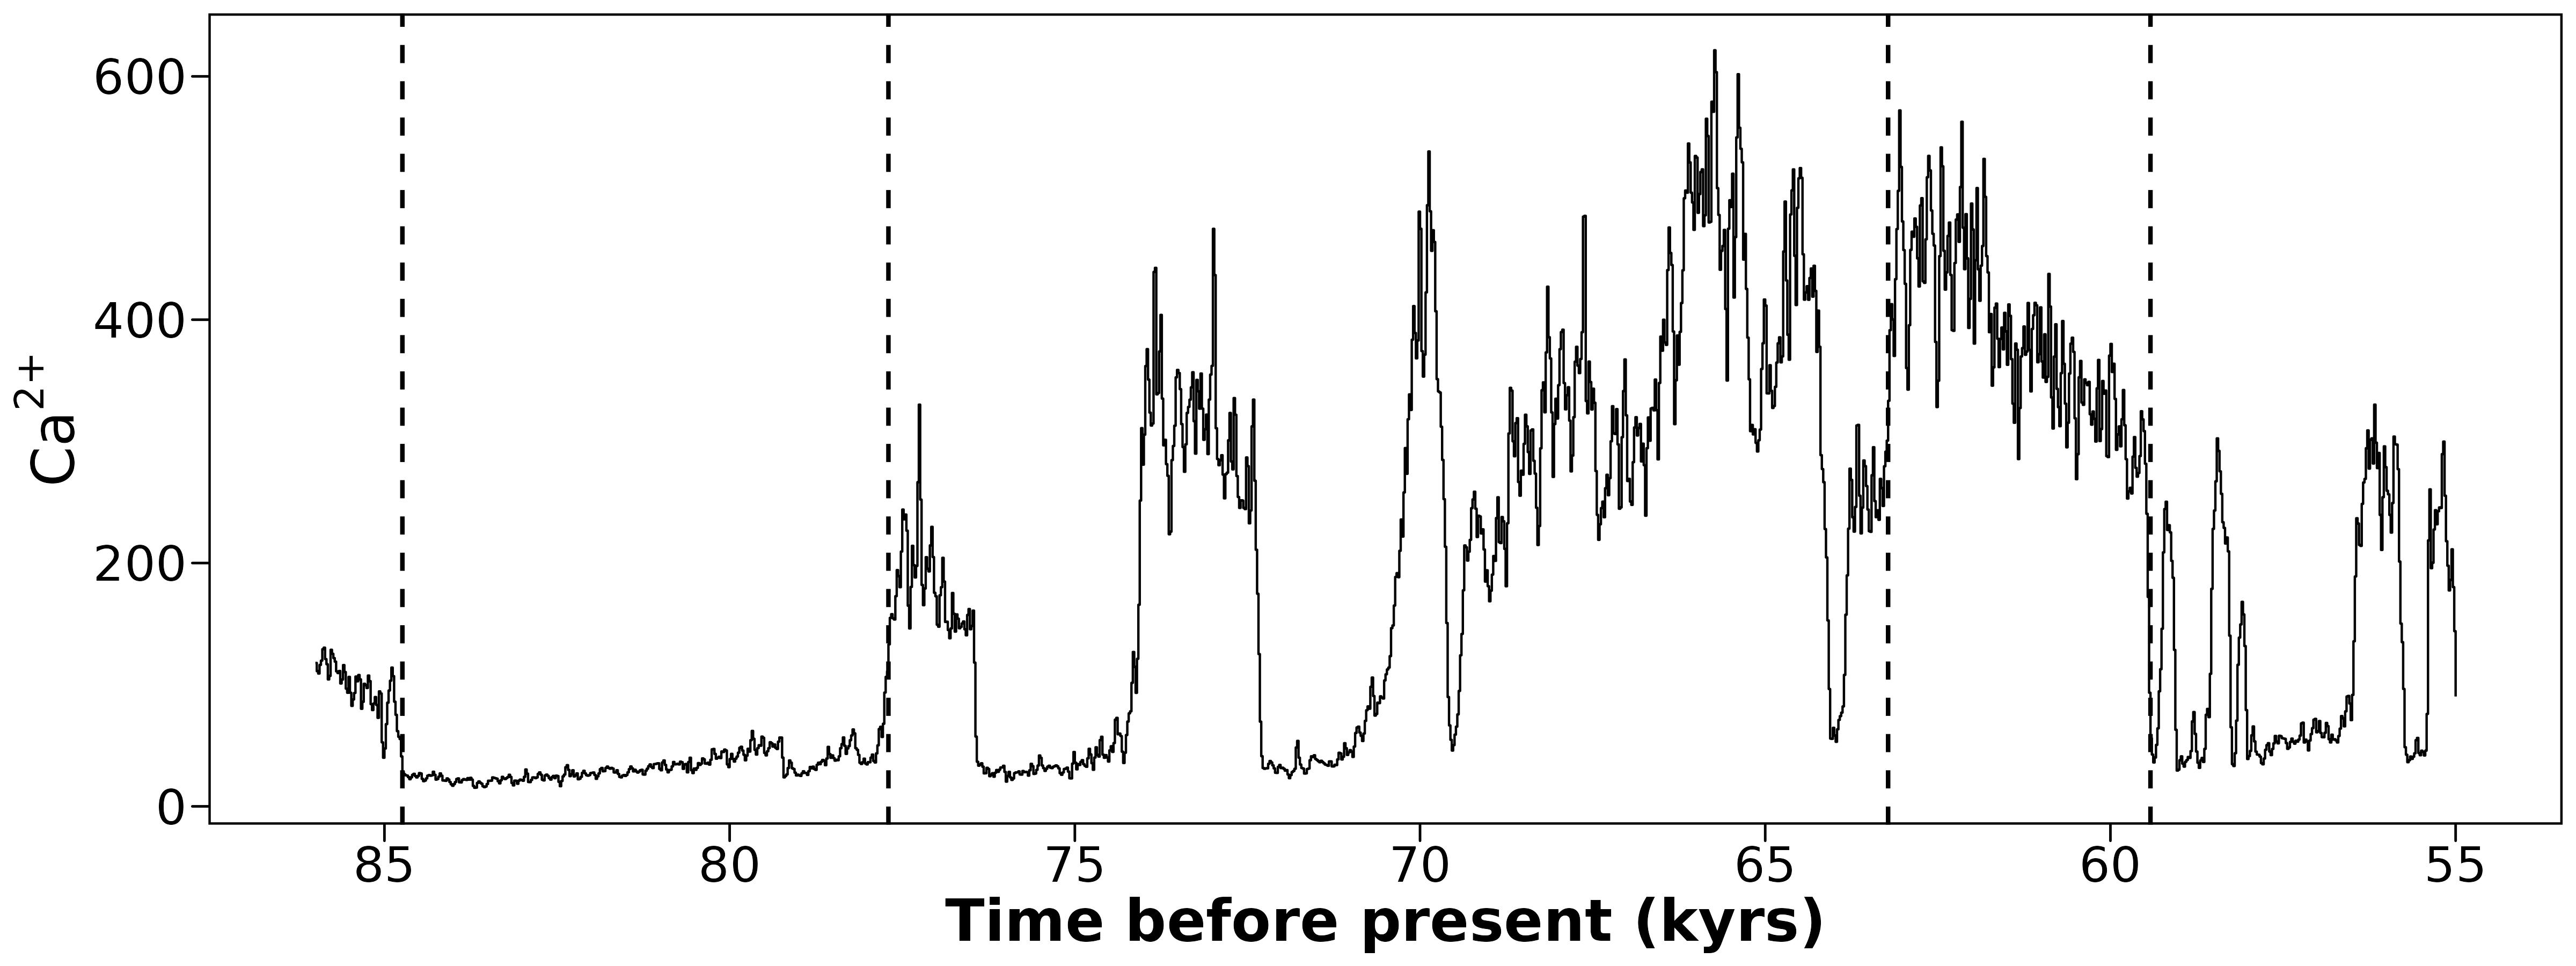
\includegraphics[scale = .075]{figures/ice_core_plot.jpeg}
%     \caption{$\mathrm{Ca}^{2+}$-concetration in the ice sheet in the periode 86 kyrs bp to 55 kyrs bp}
%     \label{figure:Ca_icesheet}
%     \end{center}
% \end{figure}\\
% Looking at graph there are some periods of time where the concetration seem to be in somewhat of a stationary state. We have marked two periods that highlights to such periods by four vertical lines. The two periods we consider concentrations for are $[77.7, 84.74]$ and $[59.42, 63.22]$; these consist of 353 and 191 observations respectively. At the end of the two periods there seem to be a tipping to another state; to make this clear we zoom in on the time periods - note that we add some of the observations after tipping for illustrative purposes
% \begin{figure}[h!]
%     \begin{center}
%     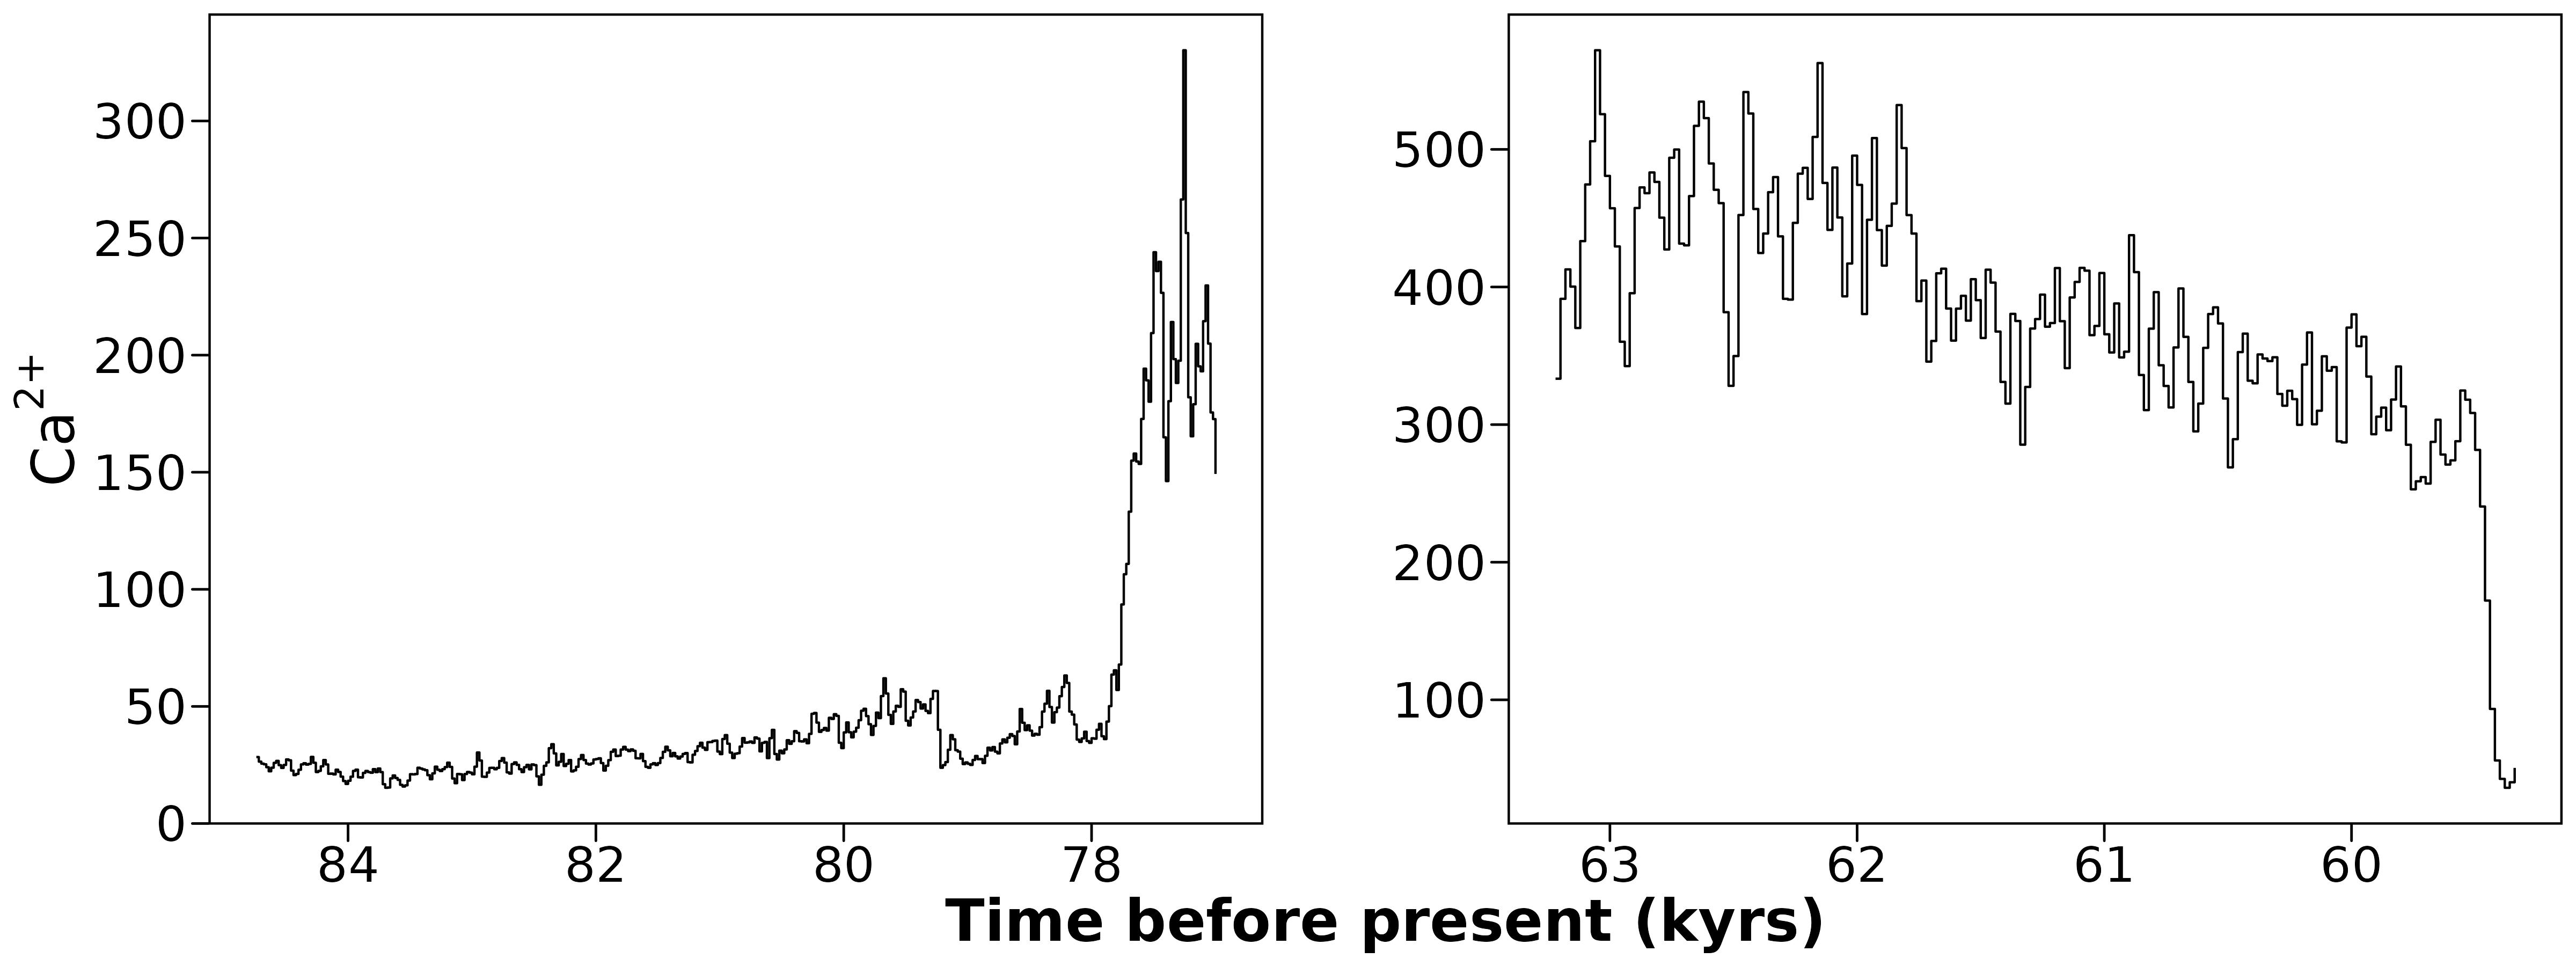
\includegraphics[scale = .075]{figures/ice_core_zoom_plot.jpeg}
%     \caption{Zoom in on the $\mathrm{Ca}^{2+}$-concetration in the ice sheet in the two intervals of interest}
%     \label{figure:Ca_icesheet}
%     \end{center}
% \end{figure}\\
% We analyze both these periods using the mean-reverting geometric brownian motion based model.